%Version 3 October 2023
% See section 11 of the User Manual for version history
%
%%%%%%%%%%%%%%%%%%%%%%%%%%%%%%%%%%%%%%%%%%%%%%%%%%%%%%%%%%%%%%%%%%%%%%
%%                                                                 %%
%% Please do not use \input{...} to include other tex files.       %%
%% Submit your LaTeX manuscript as one .tex document.              %%
%%                                                                 %%
%% All additional figures and files should be attached             %%
%% separately and not embedded in the \TeX\ document itself.       %%
%%                                                                 %%
%%%%%%%%%%%%%%%%%%%%%%%%%%%%%%%%%%%%%%%%%%%%%%%%%%%%%%%%%%%%%%%%%%%%%

%%\documentclass[referee,sn-basic]{sn-jnl}% referee option is meant for double line spacing

%%=======================================================%%
%% to print line numbers in the margin use lineno option %%
%%=======================================================%%

%%\documentclass[lineno,sn-basic]{sn-jnl}% Basic Springer Nature Reference Style/Chemistry Reference Style

%%======================================================%%
%% to compile with pdflatex/xelatex use pdflatex option %%
%%======================================================%%

%%\documentclass[pdflatex,sn-basic]{sn-jnl}% Basic Springer Nature Reference Style/Chemistry Reference Style


%%Note: the following reference styles support Namedate and Numbered referencing. By default the style follows the most common style. To switch between the options you can add or remove “Numbered” in the optional parenthesis. 
%%The option is available for: sn-basic.bst, sn-vancouver.bst, sn-chicago.bst%  
 
%%\documentclass[sn-nature]{sn-jnl}% Style for submissions to Nature Portfolio journals
%%\documentclass[sn-basic]{sn-jnl}% Basic Springer Nature Reference Style/Chemistry Reference Style
\documentclass[sn-mathphys-num]{sn-jnl}% Math and Physical Sciences Numbered Reference Style 
%%\documentclass[sn-mathphys-ay]{sn-jnl}% Math and Physical Sciences Author Year Reference Style
%%\documentclass[sn-aps]{sn-jnl}% American Physical Society (APS) Reference Style
%%\documentclass[sn-vancouver,Numbered]{sn-jnl}% Vancouver Reference Style
%%\documentclass[sn-apa]{sn-jnl}% APA Reference Style 
%%\documentclass[sn-chicago]{sn-jnl}% Chicago-based Humanities Reference Style

%%%% Standard Packages
%%<additional latex packages if required can be included here>

\usepackage{graphicx}%
\usepackage{multirow}%
\usepackage{amsmath,amssymb,amsfonts}%
\usepackage{amsthm}%
\usepackage{mathrsfs}%
\usepackage[title]{appendix}%
\usepackage{xcolor}%
\usepackage{textcomp}%
\usepackage{manyfoot}%
\usepackage{booktabs}%
\usepackage{algorithm}%
\usepackage{algorithmicx}%
\usepackage{algpseudocode}%
\usepackage{listings}%
%%%%
\usepackage{anyfontsize}

%%%%%=============================================================================%%%%
%%%%  Remarks: This template is provided to aid authors with the preparation
%%%%  of original research articles intended for submission to journals published 
%%%%  by Springer Nature. The guidance has been prepared in partnership with 
%%%%  production teams to conform to Springer Nature technical requirements. 
%%%%  Editorial and presentation requirements differ among journal portfolios and 
%%%%  research disciplines. You may find sections in this template are irrelevant 
%%%%  to your work and are empowered to omit any such section if allowed by the 
%%%%  journal you intend to submit to. The submission guidelines and policies 
%%%%  of the journal take precedence. A detailed User Manual is available in the 
%%%%  template package for technical guidance.
%%%%%=============================================================================%%%%

%% as per the requirement new theorem styles can be included as shown below
%\theoremstyle{thmstyleone}%
\newtheorem{theorem}{Theorem}%  meant for continuous numbers
%%\newtheorem{theorem}{Theorem}[section]% meant for sectionwise numbers
%% optional argument [theorem] produces theorem numbering sequence instead of independent numbers for Proposition
\newtheorem{proposition}[theorem]{Proposition}% 
%%\newtheorem{proposition}{Proposition}% to get separate numbers for theorem and proposition etc.

%\theoremstyle{thmstyletwo}%
\newtheorem{example}{Example}%
\newtheorem{remark}{Remark}%

%\theoremstyle{thmstylethree}%
\newtheorem{definition}{Definition}%

\raggedbottom
%%\unnumbered% uncomment this for unnumbered level heads

\begin{document}

\title[A $Dst$-based space weather conditions machine learning classification  model for GNSS PNT performance analysis]{A $Dst$-based space weather conditions machine learning classification  model for GNSS PNT performance analysis}

\author[1,2]{\fnm{Lucija} \sur{Žužić}}\email{lucija.zuzic@uniri.hr}
\equalcont{These authors contributed equally to this work.}

\author[1,2]{\fnm{Deni} \sur{Klen}}\email{deni.klen@uniri.hr}
\equalcont{These authors contributed equally to this work.}

\author[3]{\fnm{Teodor B.} \sur{Iliev}}\email{tiliev@uni-ruse.bg}

\author*[1,2,4]{\fnm{Renato} \sur{Filjar}}\email{renato.filjar@uniri.hr}

\affil*[1]{\orgdiv{Department of Computer Engineering}, \orgname{Faculty of Engineering, University of Rijeka}, \orgaddress{\street{Vukovarska 58}, \city{Rijeka}, \postcode{51000}, \state{Primorje-Gorski Kotar County}, \country{Croatia}}}

\affil[2]{\orgdiv{Center for Artificial Intelligence and Cybersecurity}, \orgname{University of Rijeka}, \orgaddress{\street{Radmile Matejcic 2}, \city{Rijeka}, \postcode{51000}, \state{Primorje-Gorski Kotar County}, \country{Croatia}}}

\affil[3]{\orgdiv{Department of Telecommunication}, \orgname{University of Ruse}, \orgaddress{\street{8 Studentska str.}, \city{Ruse}, \postcode{7017}, \country{Bulgaria}}}

\affil[4]{\orgdiv{Laboratory for Spatial Intelligence}, \orgname{Hrvatsko Zagorje Krapina University of Applied Sciences}, \orgaddress{\street{Setaliste hrvatskog narodnog preporoda 6}, \city{Krapina}, \postcode{49000}, \state{Krapina-Zagorje County}, \country{Croatia}}}

\abstract{Ambient conditions classification enables systematic mitigation of adversarial effects on the Global Navigation Satellite System (GNSS) Positioning, Navigation, and Timing (PNT) performance. This research contributes to the problem by proposing a classification model of space weather events for sub-equatorial regions. The proposed model uses machine learning-based classification applied to the experimental observations of geomagnetic field components, observed Total Electron Content ($TEC$), and Disturbance Storm-Time ($Dst$) index. A Support Vector Machine (SVM) with a Polynomial Kernel, C5.0 Decision Tree (DT), Naive Bayes (NB), Neural Network (NN), Partial Least Squares (PLS), Flexible Discriminant Analysis (FDA), and Neural Network using Principal Component Analysis was applied to develop the candidate model to classify observations of the geomagnetic field in $TEC$, combined with other variables, into one of the scenarios of space weather conditions. Performance is assessed using a confusion matrix and development time to yield the Naive Bayes as the best performer. The proposed $Dst$-based classification model serves as an indicator of a geomagnetic/ionospheric storm in progress, thus alerting GNSS users of a potential degradation in GNSS PNT performance and setting up a framework for the development of a tailored GNSS ionospheric correction model for specific classes of the space weather conditions.}

\keywords{Global Navigation Satellite System (GNSS) Positioning, Navigation, and Timing (PNT), space weather conditions, machine learning, classification model, decision tree (DT), neural network (NN), sensor observations aggregation, geomagnetic field, Total Electron Content (TEC), Disturbance Storm-Time (Dst) index}

%%\pacs[JEL Classification]{D8, H51}

%%\pacs[MSC Classification]{35A01, 65L10, 65L12, 65L20, 65L70}

\maketitle

\section{Introduction}
%\label{sec:Intro}

The Global Navigation Satellite System (GNSS) and its Positioning, Navigation, and Timing (PNT) service have matured to become an essential part of national infrastructure, public goods, and enablers of a vast number of emerging technology and socio-economic applications [1]. Maintaining the GNSS PNT quality has appeared fundamental for the sustainable development of modern economy and society [1]. Overcoming the shortcomings and vulnerabilities of GNSS PNT is a scientific challenge, and the need of a wide variety of scientists, developers, operators, regulators, and users of GNSS-based systems and services [2, 1]. The Earth’s ionosphere, a part of the Earth’s atmosphere stretching from 50 km to 2000 km above the Earth’s surface and comprised of rare but mostly charged atoms and molecules, is the major natural cause of GNSS PNT degradation [3, 4]. This phenomenon especially affects most currently used GNSS receivers, which work as single-frequency receivers exposed to GNSS ionospheric effects [5, 1]. Driven by powerful and random flows of energy and particles from the Sun (space weather conditions), the ionospheric conditions define the properties of GNSS signal propagation through the Earth’s atmosphere and the resulting ionospheric delay [3, 6, 4]. The GNSS ionospheric delay causes errors in GNSS PNT algorithm deployment, designed to produce position, velocity, and time estimates for a GNSS receiver [5, 4]. The ionosphere affects GNSS satellite signals for position estimation by introducing signal propagation delay [5, 4]. The GNSS ionospheric delay is a stochastic variable, whose value is determined by complex physical processes of space weather [4, 1]. How space weather affects GNSS PNT performance was explained using the Space weather – GNSS PNT performance coupling model [4], as depicted in Table~\ref{tab:Space weather – GNSS PNT performance coupling model}

\begin{table}[!ht]
    \centering
    \caption{The Space weather – GNSS PNT performance coupling model, after [4].}
    \label{tab:Space weather – GNSS PNT performance coupling model}
    \begin{tabular}{|c|c|c|c|c|}
        \hline
        % & & & & \\
        SPACE & GEOMAGNETIC & IONOSPHERE & GNSS & GNSS \\
        WEATHER & FIELD & & PSEUDO- & POSITIONING \\
         & & & RANGES & PERFORMANCE \\
        % & & & & \\
        \hline
    \end{tabular}
\end{table}

The GNSS signal encounters a certain number of charged particles from the satellite aerial to a mobile unit’s (GNSS receiver’s) aerial [4, 4]. Such an encounter is quantified using the Total Electron Content ($TEC$) defined by Equation~1 in $electrons/m^{2}$  [4, 3], where $h$ denotes the height above the Earth’s mean sea level in $m$, $N(h)$ represents the vertical ionospheric profile, the volume density of charged particles at height $h$, in $electrons/m^{2}$.

\begin{equation}
	TEC = \int_{lower \quad ionsopheric \quad boundary}^{upper \quad ionsopheric \quad boundary}N(h)dh
	\quad\left(1\right)
\end{equation}

It should be noted that in the sense of Equation~1, $TEC$ is defined as a result, a consequence, of the ionospheric conditions, and not their descriptor [1]. The GNSS ionospheric delay may be determined by derivation from the Appleton-Hartree equation, as given in Equation~2, where $\Delta t_{iono}$ denotes the GNSS ionospheric delay in $s$, $c$ denotes the velocity of an electromagnetic wave in vacuum in $m/s$, and $f$ denotes the carrier wave frequency of the satellite signal in $Hz$ [5, 4].

\begin{equation}
	\Delta t_{iono} = \frac{40.3}{c f^{2}} \int_{lower \quad ionsopheric \quad boundary}^{upper \quad ionsopheric \quad boundary}N(h)dh
	\quad\left(2\right)
\end{equation}

Combining Equation~1 and Equation~2, one can conclude the linear relation between $\Delta t_{iono}$ and $TEC$, as given in Equation~3, a sub-model incorporated in the Space weather – GNSS PNT performance coupling model [4].

\begin{equation}
	\Delta t_{iono} = \frac{40.3}{c f^{2}} TEC
	\quad\left(3\right)
\end{equation}

The GNSS ionospheric delay has been identified as a source of GNSS PNT degradation since the dawn of GNSS. GNSS systems offer various standard GNSS ionospheric delay estimation (correction) models to mitigate the deteriorating effects on GNSS PNT, such as the Klobuchar model [5, 4]. The standard ionospheric correction models are global, and insufficiently flexible to update to mitigate GNSS ionospheric delay to satisfy rising demands on GNSS PNT performance [2, 4]. The development of regional and local models attempts to solve the problem of GNSS PNT sustainable performance in various ionospheric conditions [7]. In recent developments, our team has proposed the Ambient-Aware Application-Aligned (AA)2 PNT to take into account the actual ionospheric and geomagnetic conditions near a mobile unit (a GNSS receiver) [1, 4, 2]. Direct measurements of the immediate geomagnetic and ionospheric condition variables may be supplied to a machine learning-based adapted GNSS ionospheric correction model, thus solving the single-frequency GNSS problem [1]. Previous research has identified predictors and target variables (descriptors of geomagnetic, ionospheric, and GNSS PNT conditions) [4, 8, 9]. The classification of different scenarios of GNSS ionospheric conditions with adverse effects on the GNSS PNT remained an unsolved precondition needed for the development of a machine learning-based GNSS ionospheric delay correction model to render the GNSS PNT algorithm ionospheric conditions-agnostic [1, 2].

Here we propose a methodology for a machine learning-based classification of the ionospheric conditions based entirely on observations of geomagnetic indices. The proposed method is inspired by previous lightweight machine-learning techniques [10] for classifying sensor readings. The model is sufficiently simple to be applied on computationally capable platforms with suitable geomagnetic field sensors, such as smartphones and connected/autonomous vehicles. The research presented acquires the ambient data and analyses its statistical properties. The data set is split into training and test sets. Several candidates for the GNSS ionospheric delay model are developed in this study. A tailored set of validation methods is used to assess their performance. The optimal GNSS ionospheric delay correction model is identified based on GNSS PNT-related objective criteria, and its performance is demonstrated in an independent case study.

The main contributions of this paper are:

\begin{itemize}
    \item Defining multiple $Dst$-based classes using theoretical knowledge and statistics
    \item Classifying values of $TEC$ and other geomagnetic field variables based on $Dst$
    \item Proposing a machine learning-based classification model of space weather events
    \item Achieving an accuracy over $99\%$ for the Naive Bayes model and any input variables
\end{itemize}

The findings indicate the classification generated by the Naive Bayes model could be used in real-life systems and support our hypothesis.

The rest of the paper is structured as follows. Section~\ref{sec:Dataset} describes this work's methodology, dataset, and evaluation metrics. Section~\ref{sec:Results} presents the results obtained in this study. Section~\ref{sec:Discussion} discusses the implications of the results. The main points are summarised and the conclusion is given in Section~\ref{sec:Conclusion}.

\section{Method and Data}
\label{sec:Dataset}

\subsection{Method}
%\label{subsec:Method}

A Support Vector Machine (SVM) with a Polynomial Kernel, C5.0 Decision Tree (DT), Naive Bayes (NB), shallow Neural Network (NN), Partial Least Squares (PLS), Flexible Discriminant Analysis (FDA) and shallow Neural Network using Principal Component Analysis (PCA) of the input data were tested based on their ability to classify a set of observations of the geomagnetic field in $TEC$, and other predictors, into one of the scenarios of space weather conditions based on $Dst$. Multiple $Dst$-dependent classes were predefined using theoretical knowledge. Statistical analysis of the data confirmed that distributions of other variables change for different $Dst$ ranges, and not for different $TEC$ ranges, supporting the validity of the classification. The study assumes that the dependent output variable, the $Dst$ class, can be predicted based on the independent variables used as input.

The models were selected because they represent larger families of classification methods. SVMs are supervised maximum margin models. Decision Trees also apply supervised learning. Naive Bayes classifiers are probabilistic classifiers that can be parametric or non-parametric, but this study uses a non-parametric approach. PLS is a non-parametric linear regression model. FDA uses multiple non-parametric linear regression models to create a non-linear classification. PCA is a linear dimensionality reduction technique that extracts a predefined number of components for training a Neural Network. Neural Networks imitate the brain using artificial neurons to produce outputs based on the input and the activation function. Neural Networks require that the model structure be predefined, and hyperparameters are usually tuned or predefined based on assumptions. An automated tuning procedure was used in this study.

All Neural Network models were applied based on research by Kuhn for the \textit{R} \textit{caret} package [11, 12, 13].

\subsubsection{Support Vector Machine}
%\label{subsubsec:SVM}

In machine learning, Support Vector Machines (SVMs) or Support Vector Networks (SVNs) are supervised maximum margin models with associated learning algorithms that analyze data for classification and regression. In addition to linear classification, SVMs are also effective for non-linear classification using the hyperplane kernel trick [14], implicitly mapping their inputs to high-dimensional feature spaces.

SVMs can also be used for regression tasks where the objective becomes $\epsilon$ -sensitive. A "soft margin" to separate data that is not linearly separable was proposed by Corinna Cortes and Vapnik in 1993 and published in 1995 [15]. Support Vector Clustering [16] (SVC) applies support vector statistics to unlabeled data in unsupervised learning to find new natural groupings. Meyer, Leisch, and Hornik compared SVM with other classifiers [17], but it is unclear whether SVM predictions perform better than other linear models, such as logistic, and linear regression.

Support Vector Machine constructs a set of hyperplanes in a high-dimensional space, used for classification, regression, or outlier detection [18]. Intuitively, a good separation is achieved by the hyperplane with the greatest distance to the nearest point in the training data belonging to any class [19].

The original maximum margin hyperplane algorithm proposed by Vapnik in 1963 constructed a linear classifier. In 1992, Bernhard Boser, Isabelle Guyon, and Vladimir Vapnik proposed creating nonlinear classifiers using the kernel trick [14, 20]. A multidimensional feature space increases the generalization error of Support Vector Machines, so additional samples are needed to enhance performance [21]. To keep the computational burden reasonable, a kernel probability density function $k(x, y)$ is chosen to fit the problem [22].

SVMs have been used to solve a variety of real-world problems. SVMs are useful in text and hypertext categorization, as their application can significantly reduce the need for labeled training instances in standard inductive and transductive settings [23]. Some methods for shallow semantic parsing are based on SVMs [24]. Image classification and segmentation can also be performed using SVM models, including a modified version of SVM that uses privileged access as proposed by Vapnik [25, 26].

Classification of satellite data such as Synthetic Aperture Radar (SAR) data is possible using a supervised SVM [27]. Handwritten characters can be recognized using SVM [28, 29]. The SVM algorithm is widely used in biological and other sciences. They were used to classify proteins with up to $90\%$ compounds correctly classified. Permutation tests based on SVM weights have been proposed as a mechanism for interpreting SVM models [30, 31]. SVM weights were also used to interpret SVM models [32].

The performance of SVM depends on the kernel probability density function, the parameters of the specified kernel probability density function, and the "soft" margin parameter $\lambda$. Each combination of parameter choices is usually cross-validated, and the parameters with the best accuracy are selected. The final model is used to test and classify new data and is trained using the best parameters [33].

\subsubsection{Decision Tree}
%\label{subsubsec:DT}

Decision Trees are an approach to supervised learning in statistics, data mining, and machine learning. They represent predictive or decision-making model used to make inferences about a series of observations. Tree models in which the target variable can take on a discrete set of values are called classification trees. Decision Trees where the target variable can take on continuous values (usually real numbers) are called regression trees. A regression tree can be extended to any object with pairwise differences such as categorical arrays [34]. Decision Trees are among the most popular machine learning algorithms due to their comprehensibility and simplicity [35]. A Decision Tree describes the input data and the resulting classification tree can be the input for decision-making in data mining [36].

A tree is built by dividing the original set, which forms the root node, into subsets that form descendants, or successors. The segmentation is made using a set of rules based on classification features [37]. This process is repeated on each derived subset in a recursive manner called recursive partitioning. The recursion is complete when the subset at a node all have the same target variable values or the division no longer adds value to the predictions. This process of Top-Down Induction of Decision Trees (TDIDT) [38] is an example of a greedy algorithm and is by far the most common strategy for learning Decision Trees from data [39]. C5.0, used in the \textit{caret} package in R, has a similar approach and improves the ID3 and C4.5 algorithms.

Decision Trees can also be described as a combination of mathematical and computational techniques that help describe, categorize, and generalize a given data set in data mining. Data comes in records of the form $(x, Y) = (x_{1}, x_{2}, x_{3}, \ldots, x_{k}, Y)$. The dependent variable $Y$ is the target variable we need to understand, classify, or generalize. Features $x_{1}, x_{2}, x_{3}, \ldots, x_{k}$ form the vector $X$ used for that task.

\subsubsection{Naive Bayes}
%\label{subsubsec:NB}

In statistics, Naive Bayes (NB) classifiers are a family of linear "probabilistic classifiers" that assume that, given a target class, the features are conditionally independent. The classifier got its name from this strong and possibly naive assumption. These classifiers are among the simplest Bayesian network models [40]. Naive Bayes classifiers are highly scalable and require several parameters. The number of parameters depends linearly on the number of variables. Variables represent features or predictors in the learning problem. Maximum likelihood training can be performed by evaluating a closed-form expression [41], which requires linear time, instead of the expensive iterative approximation used for many other classifiers.

In the statistical literature, Naive Bayes models are known by various names, including simple Bayes and independent Bayes [42]. These names refer to Bayes' theorem in the classifier's decision rule, but a Naive Bayesian classifier is not necessarily a Bayesian method [41, 42]. In other words, one can work with a Naive Bayesian model without accepting Bayesian probability or methods. In many practical applications, parameter estimation for Naive Bayes models uses the maximum likelihood method.

Despite their simple design and seemingly oversimplified assumptions, Naive Bayes classifiers have performed quite well in many complex real-world situations. In 2004, an analysis of the Bayesian classification problem showed that there are reasonable theoretical reasons for the seemingly incredible performance of Naive Bayesian classifiers [43]. However, a comprehensive comparison with other classification algorithms in 2006 showed that Bayesian classification performed worse than other approaches, such as boosted trees or random forests [44]. The advantage of Naive Bayes is that it requires only a small amount of training data to estimate the parameters needed for classification [45].

In the abstract, Naive Bayes is a conditional probability model. The model assigns probabilities $p(C_{k}\mid x_{1},\ldots, x_{n})$ to each of the $K$ possible outcomes or classes $C_{k}$ given the problem instance to be classified, represented by the vector $x = (x_{1},\ldots, x_{n})$ which encodes $n$ features representing mutually independent variables [46]. The problem with the above formulation is that if the number of features $n$ is large or the feature has a large value range, it is infeasible to base a model on probability tables. The model must therefore be reformulated using conditional probability represented by Bayes' theorem in Equation~4.

\begin{equation}
	p(C_{k}\mid \mathbf{x})={\frac{p(C_{k})\ p(\mathbf{x} \mid C_{k})}{p(\mathbf{x})}}
	\quad\left(4\right)
\end{equation}

To estimate feature distribution parameters, we must assume a parametric distribution, or generate non-parametric models for the features from the training data set [47]. Assumptions about the distribution of features are called an event model or Bayesian classifier, which can introduce confusion by creating both a continuous and discrete model [48, 49]. Multinomial and Bernoulli distributions have often been used for discrete features in document classification, or spam filtering. The Gaussian Naive Bayesian classifier was used since the features used in this study assumed continuous values.

Clustering is often used to discretize continuous values. The new set of features obtained by discretization follows the Bernoulli distribution. Some literature claims that discretization is necessary to use a Naive Bayesian classifier, but discretization may discard the information needed to distinguish between classes [42].

Sometimes the distribution of class-based marginal densities is far from normal. The marginal probability density of each class can be used to estimate the kernel probability density function in such cases. This method, introduced by John and Langley [47], can significantly increase the accuracy of the classifier [50, 19].

\subsubsection{Neural Networks}
%\label{subsubsec:NN}

The neurons of human or animal brains provide the basis for a Neural Network (NN) or Artificial Neural Network (ANN) with connected units or nodes called artificial neurons in machine learning [51, 52]. 

Shallow Neural Networks are simple and easy to train quickly with fewer parameters, and computational resources. They typically contain only a few hidden layers for processing between the input layer that receives the data, and the final layer that produces the output [53, 54].  A network with at least two hidden layers [55] is considered a deep Neural Network.

Neural Networks are typically trained through empirical risk minimization. This method optimizes the network's parameters to minimize the difference or empirical risk, between the predicted output and the actual target values in a given dataset [56]. Gradient-based methods such as backpropagation are usually used to estimate network parameters  [56]. During the training phase, ANNs learn from labeled training data by iteratively updating their parameters to minimize a defined loss function [57].

Using Artificial Neural Networks requires an understanding of their characteristics. The model suitable for a specific task varies depending on how the data is stored and other practical considerations. Many model parameters may need to be adjusted and differ for each model. The hyperparameters for the learning algorithm may also be modified to suit the problem [58] during an extensive tuning process experimenting on unseen training data, and various learning algorithms are available.

The network design process can be simplified using previously defined machine learning techniques like neural architecture search (NAS). These networks have performed well even when pitted against architectures selected by humans. The proposed model is tested and the responses are used to train the NAS network [59]. AutoML and AutoKeras [60] provide extensive frameworks for this process. The \textit{scikit-learn} library features various classification, regression, and clustering algorithms including support-vector machines, random forests, gradient boosting, k-means, and Density-Based Spatial Clustering (DBSCAN). The hyperparameters must be predefined, are not trained, and include how many neurons are in each layer, learning rate, step, stride, depth, receptive field, and padding for CNNs [61]. TensorFlow and Keras are used to build a custom network in Python, and the user can define layers, models, or metrics. The data, number of hidden layer units, learning rate, and number of iterations are required parameters for model training based on a book by Liu [62].

\subsubsection{Partial Least Squares}
%\label{subsubsec:PLS}

Partial Least Squares (PLS) regression, or projection to latent structures, [63, 64], is a linear regression statistical model that transforms the predicted and the observable variables to a new space instead of identifying maximum variance hyperplanes used in a linear regression model. Svante and Herman O. A. Wold, a Swedish father and son, founded this approach. PLS methods are bilinear factor models because the $X$ and $Y$ are projected to new spaces. In Partial Least Squares Discriminant Analysis (PLS-DA), $Y$ is categorical [65].

Using $n$ paired observations $\left(\vec{x_{i}}, \vec{y_{i}}\right), i \in 1, \dots, n$. PLS finds the normalized direction $\vec{p_{j}}, \vec{q_{j}}$ that maximizes the covariance in the first step $j = 1$ [66], shown in Equation~5. Matrix notation is used in further discussion of the model.

\begin{equation}
	\max_{{\vec{p}}_{j},{\vec{q}}_{j}}\operatorname{E} [\underbrace{({\vec{p}}_{j}\cdot {\vec{X}})}_{t_{j}}\underbrace{({\vec{q}}_{j}\cdot {\vec{Y}})}_{u_{j}}
	\quad\left(5\right)
\end{equation}

The scores form an orthogonal basis in PLS regression, and the loadings are chosen to achieve this. In Principal Component Analysis (PCA) orthogonality is not imposed on scores but onto loadings instead [67, 68, 69, 70, 71, 64]. Many versions of PLS exist for estimating the factor and loading matrices, such as the PLS1 algorithm [72, 73]. 

\subsubsection{Flexible Discriminant Analysis}
%\label{subsubsec:FDA}

Flexible Discriminant Analysis (FDA) is a general methodology that creates the discriminant surface for a multigroup non-linear classification model based on a mixture of non-parametric linear regression models [74], such as Multivariate Adaptive Regression Splines (MARS) and linear discriminant analysis (LDA).

Many predictors can be used at once in FDA [75], variable interactions are automatically noted [76], it is complex but execution time and computational load are adequate [77]. The algorithm is not significantly affected by outliers [78].

Modifying different settings has a high impact on FDA [79], and the estimation might be unsuccessful if the predictor distributions are highly correlated. FDA is prone to overfitting [80], and challenging to comprehend or explain [81]. The assumption of normality for the continuous independent variables is necessary [82] to determine the response or grouping categorical variable. 

Linear discriminant analysis (LDA), normal discriminant analysis (NDA), or discriminant function analysis is a generalization of Fisher's linear discriminant defined in 1936 [83]. The results of LDA may be utilized directly or to reduce dimensionality before classification, which is more often used [84]. LDA finds a linear combination of features or measurements differentiating two or more sample classes [85, 86]. Discriminant analysis has continuous independent variables and a categorical dependent variable representing the groups [87].

LDA is closely related to PCA and factor analysis since they identify linear functions of multiple variables that fit the input with the smallest error [88]. Discriminant correspondence analysis [89, 90] is equivalent to LDA for categorical independent variables. Points in discriminant function analysis are rated based on quantitative predictors and a group measure [91] to represent classification [92].

The assumptions of MANOVA are also true for discriminant analysis. The analysis is highly affected by outliers so there must be fewer predictor variables than samples in the smallest class [91]. In every level of the grouping variable, independent variables must be normal to achieve multivariate normality [91, 84]. Box's M statistic [84] test whether homogeneity of variance/covariance is established and whether variances among group variables change for predictor levels. 

Quadratic instead of linear discriminant analysis should be utilized if covariances are different [91]. The scores of one predictor variable should not depend on other predictor variables for any sample, and the samples should be chosen at random [91, 84]. Discriminant analysis can handle small deviations from these requirements [93] and may be used even if multivariate normality is not achieved, such as for dichotomous variables [94].

The discriminant rules suggest that if $x\in \mathbb{R}_{j}$, then $x\in j$ for a group $j$, and $\mathbb{R}_{j}$ sets of sample space. The discriminant analysis method identifies regions of $\mathbb{R}_{j}$ that decrease errors of classification [95]. A discriminant score describes how well a discriminant differentiates classes. [96].
 
The discriminant analysis eigenvalue represents the characteristic root of each function, indicating the quality of the group separation produced by the function. The function differentiates better for a larger eigenvalue [91]. Eigenvalues do not have an upper limit [91, 84], so the results should not be taken at face value.

Even though it is not universally accepted, some suggest eigenvalues be utilized as effect size measures [84]. The percent of correctly classified data, such as the kappa value, can also be used as the effect size while accounting for random matches in classification [84]. Kappa is not biased for any particular class, whether performance is high or low, and instead normalizes across all classes [97]. 

Fisher's linear discriminant and LDA are sometimes considered synonyms. However, Fisher [85] describes a slightly different discriminant, which does not make some of the assumptions of LDA such as a normal distribution or the equality of covariances for groups. The application of the Fisher discriminant is expanded to find a subspace capturing all class variability [96] for multiple groups, as suggested by C. R. Rao [98].

\subsubsection{Principal Component Analysis}
%\label{subsubsec:PCA}

Principal component analysis (PCA) is a linear dimensionality reduction technique with applications in exploratory data analysis, visualization, and data preprocessing. It is used in preprocessing before training a Neural Network in the $pcaNNe$ method in the \textit{caret} package in \textit{R} [99]. The data is linearly transformed into a new coordinate system such that the directions (principal components) capturing the largest variation in the data can be easily identified. Many studies use the first two principal components to plot the data and visually identify clusters of closely related data points [100].

PCA is closely related to factor and canonical correlation analysis (CCA). PCA is the simplest of the true eigenvector-based multivariate analyses. PCA defines a new orthogonal coordinate system that optimally describes the variance in a single dataset [101, 102, 103, 104]. CCA does the same for the cross-covariance between two datasets. Robust and L1-norm-based variants of standard PCA have also been proposed [104, 105, 106, 107].

Karl Pearson [108] conceived of PCA in 1901 as a counterpart of the principal axis theorem in mechanics [109]. Harold Hotelling discovered the Hotelling transform in multivariate quality control in the 1930s without knowledge of the previous work [110, 111]. Synonyms for PCA include the discrete proper orthogonal decomposition (POD) [112, 113, 114, 115] in mechanical engineering and the Kosambi–Karhunen–Loève or Karhunen–Loève theorem (KLT) [116, 117, 118, 119, 120, 121] in signal processing. Singular value decomposition (SVD) of X, established in the final quarter of the 19th century [122], is also similar to PCA. Eigenvalue decomposition (EVD) of a matrix $\mathbf{X}^{\mathsf{T}}\mathbf{X}$ in linear algebra shares the mathematical foundations of PCA [123, 124]. Factor analysis differs in several key features [125], but has many aspects in common with PCA. Empirical orthogonal functions (EOF) [126] in meteorological science were developed by Lorenz in 1956 [126]. The Eckart–Young theorem [127] and quasiharmonic modes [128] are both connected to PCA. Empirical modal analysis in structural dynamics and spectral decomposition in noise and vibration also take a similar approach to PCA.

The data in PCA is converted to a new coordinate system using a scalar projection, an orthogonal linear transformation on a real inner product space. The first coordinate or principal component covers the largest portion of the variance, decreasing with each following component [125, 129]. The significance of the principal components can be checked with parametric bootstrap for a smaller dataset to help decide how many principal components to keep [130].

\subsection{Data Description and Analysis}
%\label{subsec:Data}

Many parameters can describe the Earth's geomagnetic field, but this study focuses on those describing disturbances of the geomagnetic field, most importantly $K_p$, $A_p$, $TEC$, and $Dst$. The $K_p$ index quantifies global geomagnetic activity by measuring disturbances in the horizontal component of Earth's magnetic field. The $K_p$ index is based on 3-hour-based $K$ indices from 12 geomagnetic locations.

The $K$ index is defined by Table\ref{tab:K}.

\begin{table}[!ht]
    \centering
    \caption{The $K$ index.}
    \label{tab:K}
    \begin{tabular}{|c|c|}
        \hline
        Geomagnetic & The intensity of a \\ 
        observatory $K$ index & geomagnetic storm \\ \hline
        $0$ - $1$ & Quiet geomagnetic conditions \\ \hline
        $2$ - $4$ & Unsettled \\ \hline
        $5$ & Minor storm \\ \hline
        $6$ & Large storm \\ \hline
        $7$ & Severe geomagnetic storm \\ \hline
        $8$ - $9$ & Very intense (extreme) geomagnetic storm \\ \hline
    \end{tabular}
\end{table}

The $K$ index is an integer in the range $0$ to $9$ ($NGK$ lower scare is $500$, $PAF$ lower scale is $750$), the largest range of geomagnetic disturbances $a_x$ and $a_y$ in the two horizontal components $X$ and $Y$ during a $3$-hour UT interval.

The $A_p$ index is a single value of magnetic activity for the entire day, the average of $8$ $K$ indexes. 
 
Elevated $TEC$ levels can increase signal delay which can cause positioning errors, especially critical for high-precision applications. $TEC$ can be calculated as indicated in Equation~1, Equation~2, and Equation~3. 

The GPS Ionospheric delay on the radio ray path between satellite and receiver is defined in Equation~6 [5] where $\Delta t$ represents the GPS ionospheric delay, $c$ is the velocity of light, and $n(l)$ is the refraction index on the path $l$.

\begin{equation}
	\Delta t = \frac{1}{c} \int_{satellite}^{receiver} \left[ n(l) - l \right]dl
	\quad\left(6\right)
\end{equation}

The GPS ionospheric delay $\Delta \rho \dots$ related to distance measurements can be defined using Equation~7 [5].

\begin{equation}
	\Delta \rho = \frac{1}{c} \int_{satellite}^{receiver} \left[ n(l) - l \right]dl
	\quad\left(7\right)
\end{equation}

Appleton’s formula in Equation~8 reasonably approximates the relationship between the refraction index and the free electron density distribution [3, 5]. $N(h)$ is the vertical distribution of the free electron density over a height $h$ above the surface of the Earth, and $f$ is the frequency of the radio signal.

\begin{equation}
	n(l) = 1 + \frac{40.3 N(h)}{f^{2}}
	\quad\left(8\right)
\end{equation}

The combination of Equation~6 and Equation~8 yields Equation~9 that directly describes the relationship between the free electron density profile and the GPS ionospheric delay [5].

\begin{equation}
	\Delta t = \frac{40.3}{c f^{2}} \int_{receiver}^{satellite} N(h)dh
	\quad\left(9\right)
\end{equation}

The $TEC$ [5] in Equation~10 is calculated using the integral on the right side of Equation~9.

\begin{equation}
	TEC = \int_{receiver}^{satellite} N(h)dh
	\quad\left(10\right)
\end{equation}

Using equation Equation~10, Equation~9 can be written as shown in Equation~11.

\begin{equation}
	\Delta t = \frac{40.3}{c f^{2}} TEC
	\quad\left(11\right)
\end{equation}

Following the same analogy, the equivalent GPS ionospheric delay is calculated in Equation~12.

\begin{equation}
	\Delta \rho = \frac{40.3}{c f^{2}} TEC
	\quad\left(12\right)
\end{equation}

Considering the pseudo-range measurements taken on both GPS transmitting frequencies ($f_{1}=1575.42$ $MHz$ and $f_{2}=1227.60$ $MHz$) and using Equation~12, the relation between the $TEC$ and GPS pseudo-range measurements can be established in Equation~13 [5]:
 
\begin{equation}
	\rho_{1} - \rho_{2} = 40.3 TEC \left( \frac{1}{f_{1}^{2}} - \frac{1}{f_{2}^{2}} \right)
	\quad\left(13\right)
\end{equation}

Equation~13 can be rewritten as in Equation~14, defining $TEC$. The actual value of the $TEC$ can be computed utilizing a dual-frequency GPS receiver and Equation~14.

\begin{equation}
	TEC = \frac{\rho_{1} - \rho_{2}}{40.3} \frac{{\left(f_{1}f_{2}\right)}^{2}}{f_{2}^{2}-f_{1}^{2}}
	\quad\left(14\right)
\end{equation}

Considering the imposed regulations for common GPS dual-frequency receiver use, a different method for estimating the $TEC$ and GPS ionospheric delay is needed. A standard GPS ionospheric delay model, such as the Klobuchar model in Equation~15 [131, 5]. A cosine-like daily dynamic of GPS ionospheric delay values is assumed in the Klobuchar model, with the daily maximum appearing around 14:00 in local time [132].

\begin{equation}
	\Delta t = F \left[ t_{n} + A \cos \frac{2\pi\left(t-t_{0}\right)}{P} \right]
	\quad\left(15\right)
\end{equation}

The next relevant parameter is $Dst$, also known as the $Dst$ index, a measure of geomagnetic storm intensity. $Dst$ describes ring currents forming above the sub-equatorial region and affecting the ionospheric regions in mid-latitudes.

The $Dst$ index is derived from measurements taken by a network of ground-based magnetometer stations located near the magnetic equator, which continuously monitor the horizontal component of Earth's magnetic field. To calculate the $Dst$ index, variations in the horizontal magnetic field from these stations are averaged, and this average is then subtracted from a baseline value representing the quiet-time magnetic field. The resulting $Dst$ value, expressed in nanoteslas ($nT$), measures the intensity of geomagnetic disturbances, with more negative values indicating stronger geomagnetic storms. The performance of GNSS is linked to many dynamic conditions of space weather. Solar activity can induce various effects that degrade the accuracy, availability, and reliability of GNSS PNT. Incorporating parameters such as the $Kp$ and $A_p$ indexes, which provide global measures of geomagnetic activity, alongside $TEC$ and the Disturbance Storm Time ($Dst$) index, allows for a more detailed assessment of the space environment and its potential effects on GNSS signals. In this paper, $A_p$, $TEC$, and $Dst$ were used with ,$B_x$, $B_y$, and $B_z$ to train machine-learning models.

To generate classes, samples were split into $5$ ranges, P (positive, $Dst$ from $15$ to $50$), N (normal, $Dst$ from $-20$ to $15$), R (recovery, $Dst$ from $-55$ to $-20$), T (through, $Dst$ from $-85$ to $-55$), and E (extreme, $Dst$ from $-120$ to $-85$), based on $Dst$ values derived from theoretical knowledge of different storm phases. The ranges are listed in Table \ref{tab:Dstranges}.

\begin{table}[!ht]
    \centering
    \caption{$Dst$-based classification rules.}
    \label{tab:Dstranges}
    \begin{tabular}{|c|c|}
        \hline
        $Dst$ & Storm phase classification \\ \hline
        $15\dots50$ & positive phase (P) \\ \hline
        $-20\dots15$ & normal (N) \\ \hline
        $-55\dots-20$ & recovery phase (R) \\ \hline
        $-85\dots-55$ & through (T) \\ \hline
        $-120\dots-85$ & extreme (E) \\ \hline
    \end{tabular}
\end{table}

Figure~\ref{fig:correlation} contains a heat map of the correlation between all variables used in this study. Blue represents a low correlation, while red represents a higher correlation. Swapping the row and column leads to the same combination of variables, so the matrix is symmetrical concerning the secondary diagonal. The values on the secondary diagonal equal $1$ and can be disregarded because all variables are fully correlated with themselves. Besides these values on the secondary diagonal, the highest correlation of $0.78$ is between $dTEC$ and $TEC$, as expected based on previously outlined theoretical aspects of these variables. $B_{x}$ and $Dst$ have a correlation coefficient of $0.52$, the second highest value not on the secondary diagonal. This is the only other value larger than $0.5$ not on the secondary diagonal. A high correlation of $B_{x}$ and $Dst$ supports the hypothesis that we can predict $Dst$ values, ranges, or classes using $B_{x}$. The third highest correlation coefficient not on the secondary diagonal is between $B_{x}$ and $B_{y}$ and equals $0.44$. The properties and definitions of these variables explain this correlation.

\begin{figure}
 \centering
 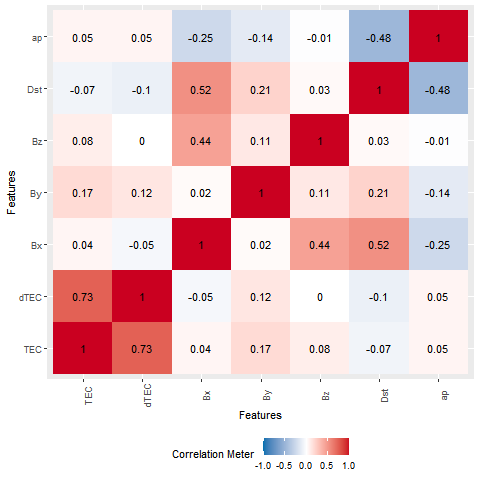
\includegraphics[width=0.9\linewidth]{correlation.png}
    \caption{A heat map of the correlation between all variables used in this study, where red represents a higher correlation, while blue represents a low correlation. All variables are fully correlated with themselves, so all values on the secondary diagonal equal $1$. The matrix is symmetrical concerning the secondary diagonal because the same combination of correlated variables is achieved when swapping the row and column.}
    \label{fig:correlation}
\end{figure}

The box plots of all variables for different ranges of $Dst$ values in Figure~\ref{fig:dataset2boxplot}, without restriction on the range of $TEC$, and in Figure~\ref{fig:iono3boxplot}, where the $TEC$ is less than $300$, demonstrate that the minimum, maximum, and arithmetic mean of $A_{p}$ decrease for larger $Dst$ values regardless of $TEC$ ranges. The opposite is true for $B_{x}$, as indicated by a high correlation of $B_{x}$ and $Dst$ in Figure~\ref{fig:correlation}. $B_{y}$ exhibits the same trend as $B_{x}$, but it is less prominent. $B_{z}$ is the most stable variable with the smallest changes related to $Dst$ when observing $B_{x}$, $B_{y}$, and $B_{z}$, but an increase for larger $Dst$ values can also be observed. Similar conclusions can be reached from the scatter plots of all variables for different ranges of $Dst$ in Figure~\ref{fig:iono3scatterplot}. 

The scatter plots of all variables for different ranges of $TEC$ values in Figure~\ref{fig:dataset2scatterplot} demonstrate that their distribution is not significantly dependent on $TEC$. This is why the box plots in Figure~\ref{fig:dataset2boxplot} and Figure~\ref{fig:iono3boxplot} that only differ in $TEC$ ranges look very similar. A minimal difference is also evident between the histograms of the relative frequency for all variables in Figure~\ref{fig:allTEC}, without restriction on the range of $TEC$, and in Figure~\ref{fig:300TEC}, where the $TEC$ is less than $300$. Table~\ref{fig:iono3boxplot} provides the minimum, $1^{st}$ quartile, median, arithmetic mean, $3^{rd}$ quartile, and maximum values for all variables, supporting the conclusions made based on Figure~\ref{fig:dataset2boxplot} and Figure~\ref{fig:allTEC}.

\begin{figure}
    \centering
    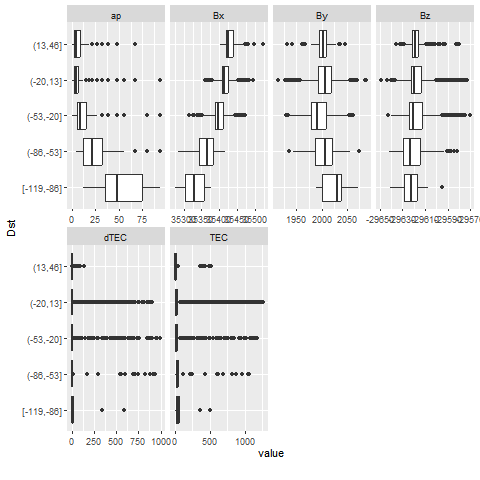
\includegraphics[width=0.9\linewidth]{dataset2boxplot.png}
    \caption{Box plots of all variables without restriction on the range of $TEC$ for different ranges of $Dst$ values defining the class label used in this study.}
    \label{fig:dataset2boxplot}
\end{figure}

\begin{figure}
    \centering
    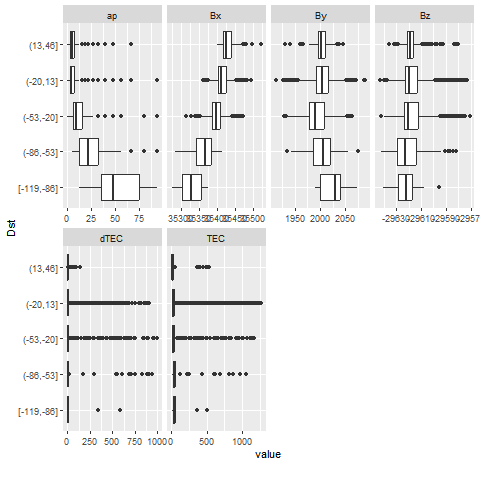
\includegraphics[width=0.9\linewidth]{iono3boxplot.png}
    \caption{Box plots of all variables when the $TEC$ is less than $300$ for different ranges of $Dst$ values defining the class label used in this study.}
    \label{fig:iono3boxplot}
\end{figure}

\begin{figure}
    \centering
    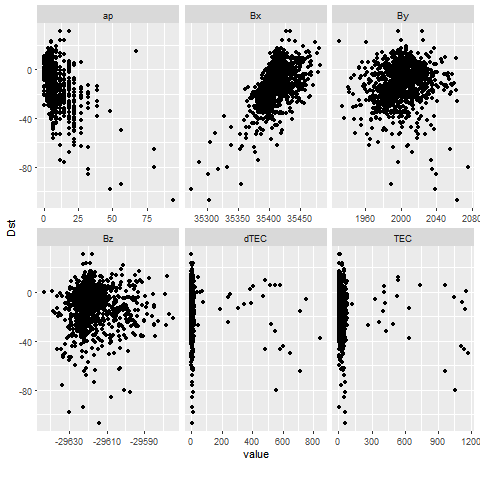
\includegraphics[width=0.9\linewidth]{iono3scatterplot.png}
    \caption{Scatter plots of all variables when the $TEC$ is less than $300$ for different ranges of $Dst$ values defining the class label used in this study.}
    \label{fig:iono3scatterplot}
\end{figure}

\begin{figure}
    \centering
    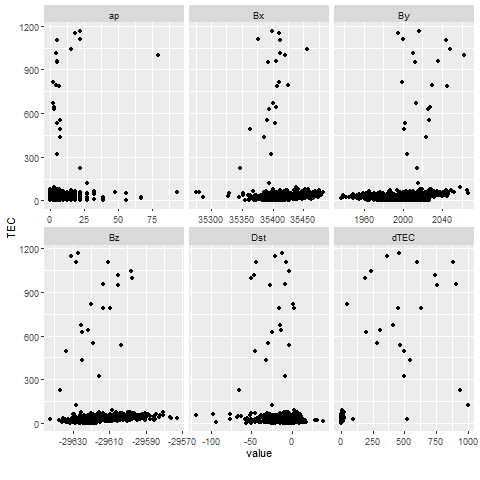
\includegraphics[width=0.9\linewidth]{dataset2scatterplot.png}
    \caption{Scatter plots of all variables for different ranges of $TEC$ values without restriction.}
    \label{fig:dataset2scatterplot}
\end{figure}

\begin{figure}
    \centering
    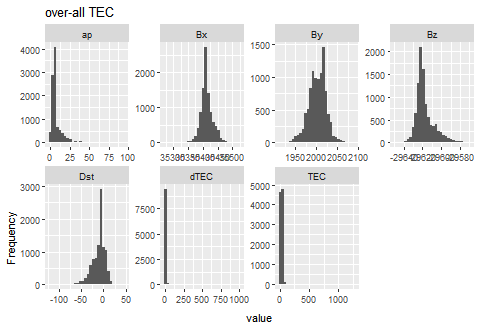
\includegraphics[width=0.9\linewidth]{allTEC_fix.png}
    \caption{Histograms of the relative frequency for all variables without restriction on the range of $TEC$.}
    \label{fig:allTEC}
\end{figure}

\begin{figure}
 \centering
 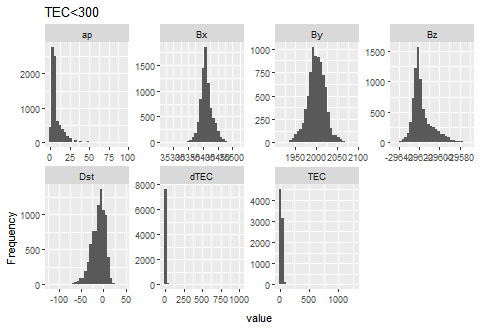
\includegraphics[width=0.9\linewidth]{300TEC_fix.png}
    \caption{Histograms of the relative frequency for all variables when the $TEC$ is less than $300$.}
    \label{fig:300TEC}
\end{figure}

\begin{table}[!ht]
    \centering
    \caption{The minimum, $1^{st}$ quartile, median, arithmetic mean, $3^{rd}$ quartile, and maximum values for all variables.}
    \label{tab:my_label}
    \begin{tabular}{|c|c|c|c|c|c|}
        \hline
        & $TEC$ & $dTEC$ & $B_{x}$ & $B_{y}$ & $B_{z}$ \\ \hline
        Min. & $1.00$ & $0.01$ & $35268$ & $1900$ & $-29651$ \\ \hline
        $1^{st}$ Qu. & $7.26$ & $1.66$ & $35400$ & $1988$ & $-29623$ \\ \hline
        Median & $19.62$ & $3.13$ & $35410$ & $2001$ & $-29620$ \\ \hline
        Mean & $40.00$ & $15.88$ & $35412$ & $2001$ & $-29617$ \\ \hline
        $3^{rd}$ Qu. & $34.23$ & $6.49$ & $35423$ & $2015$ & $-29613$ \\ \hline
        Max. & $1288.00$ & $997.00$ & $35527$ & $2092$ & $-29570$ \\ \hline
    \end{tabular}
\end{table}

\subsubsection{Data Pre-processing}
%\label{subsubsec:Pre-processing}

Data pre-processing is recommended to increase classification accuracy [133], so this step was also applied to the input data before training the models in this study. There are many ways to standardize data, such as minimum-maximum, normalization by decimal scaling, and Z-score [134]. Subtracting the mean and dividing by the variance for each feature are commonly used for Support Vector Machines (SVMs) [135] and other models tested in this study, so this approach was chosen. 

The values \textit{scale} and \textit{center} were used in the code for this study in the \textit{preProcess} parameter for the \textit{train} function from the \textit{caret} package developed for \textit{R}. The option \textit{center} subtracts the mean of each feature while \textit{center} divides by the standard deviation. 

\subsubsection{Training and Testing Dataset}
%\label{subsubsec:DataTrainTest}

The samples are divided into training and testing datasets as close as possible to a ratio of $80\%$ for training and $20\%$ for testing. During the division, the share of classes in the original data was taken into account, that is, the division was stratified by class so that an approximately equal ratio of classes was present in both the training data and the testing data, which is a feature of the \textit{createDataPartition} function from the \textit{caret} R library that was used [136, 137, 138].

\subsection{Performance Metrics}
%\label{subsec:Metrics}

\subsubsection{Confusion Matrix}
%\label{subsubsec:ConfusionMatrix}

The metrics and terminology used to evaluate the classifier performance were taken from the confusion matrix defined in the R function \textit{confusionMatrix} in the \textit{caret} library [139, 140, 141, 142, 143]. The confusion matrix is suitable for use in multiclass classification, which is the goal of this project. A confusion matrix is a table where the number of rows and columns corresponds to the number of classes. The cells report the number of samples in each class classified into any class. This enables a more detailed analysis than by observing the share of correct classifications, i.e. accuracy. Accuracy will give results that can lead us to a wrong conclusion if the data set is unbalanced, that is, if the numbers of observations in different classes vary significantly, which was the case in this paper, because out of a total of $1597$ samples, $1170$ of them belonged to the largest N class, and $3$ to the smallest E class.

If there are only two classes (Yes and No), the metrics are calculated using an example of a confusion matrix in Table~\ref{tab:cm}.

A true positive (TP) classification result correctly indicates that the sample belongs to the positive class.

A true negative (TN) classification result correctly indicates that the sample belongs to the negative class.
 
A false positive (FP) classification result or type I error, incorrectly indicates that the sample belongs to the positive class because it truly belongs to the negative class.

A false negative (FN) classification result or type II error, incorrectly indicates that the sample belongs to the negative class because it truly belongs to the positive class.

\begin{table}[!ht]
    \centering
    \caption{The confusion matrix for a two-class problem.}
	\label{tab:cm}
	\begin{tabular}{|c|c|c|}
		\hline
		 & \multicolumn{2}{|c|}{Reference} \\ \hline
        Prediction & Yes & No \\ \hline
        Yes & TP & FP \\ \hline
        No & FN & TN \\ \hline
	\end{tabular}
\end{table}

Sensitivity, recall, hit rate, or true positive rate (TPR), is calculated as $\mathrm{TP}/(\mathrm{TP}+\mathrm{FN})$, that is, the proportion of samples that are correctly classified as positive among all samples that truly belong to the positive class. Higher TPR values indicate better results for the positive class.

Specificity, selectivity, or true negative rate (TNR), is calculated using the expression $\mathrm{TN}/(\mathrm{TN}+\mathrm{FP})$, that is, the proportion of samples that are correctly classified as negative among all samples that truly belong to the negative class. Higher TNR values indicate better results for the negative class.

Prevalence is calculated as $(\mathrm{TP}+\mathrm{FN})/(\mathrm{TP}+\mathrm{FP}+\mathrm{FN}+\mathrm{TN})$ for the positive class, that is, the proportion of samples that truly belong to the positive class among all samples. Prevalence values other than an even split by the number of classes indicate a class imbalance.

Precision, or positive predictive value (PPV), is calculated as $\mathrm{TP}/(\mathrm{TP}+\mathrm{FP})$ for a two-class problem, i.e. the proportion of truly positive results among all samples classified as positive. 
Higher PPV values indicate better results for the positive class.

The negative predictive value (NPV) is calculated as $\mathrm{TN}/(\mathrm{TN}+\mathrm{FN})$ for a two-class problem, i.e. the share of truly negative results among all samples that are classified as negative. Higher NPV values indicate better results for the negative class.

The detection rate (DR) is calculated as $\mathrm{TP}/(\mathrm{TP}+\mathrm{FP}+\mathrm{FN}+\mathrm{TN})$ for the positive class, that is, that is, the proportion of samples that are correctly classified as positive among all samples.

The detection prevalence (DP) is calculated as $(\mathrm{TP}+\mathrm{FP})/(\mathrm{TP}+\mathrm{FP}+\mathrm{FN}+\mathrm{TN})$ for the positive class, that is, that is, the proportion of samples that are correctly or incorrectly classified as positive among all samples.

The accuracy (Acc) is calculated as $(\mathrm{TP} + \mathrm{TN}) / (\mathrm{TP} + \mathrm{TN} + \mathrm{FP} + \mathrm{FN})$, that is, the proportion of samples that are correctly classified among all samples.

Since accuracy is not usable in the case of unbalanced classes, balanced accuracy (BA) is introduced, which is calculated as $(\mathrm{TPR} + \mathrm{TNR}) / 2$ and is arithmetic mean TPR and TNR, which are respectively centered on the positive and on the negative class separately.

Another metric that can be used instead of accuracy to consider each class separately is the $F1$ score, i.e. the harmonic mean of PPV and TPR, equal to $2 \times (\mathrm{PPV} \times \mathrm{TPR}) / (\mathrm{PPV} + \mathrm{TPR}) = 2 \times \mathrm{TP} / (2 \times \mathrm{TP} + \mathrm{FP} + \mathrm{FN})$.

If there are more than two classes, results are calculated for each class separately by viewing that class as the positive class and samples of all other classes as negative, a "one versus all" approach.
The unweighted Kappa statistic and a \textit{p}-value from McNemar's test are also computed. McNemar's test produces NA values with sparse tables, such as the one in this experiment, so it was not included in the results.

A $95\%$ confidence interval for the accuracy rate is computed using \textit{binom.test} and a one-sided test [144, 145, 146, 147] to see if the accuracy is significantly larger than the "no information rate," which is the percentage of the largest class.

\subsubsection{The Binomial Test}
%\label{subsubsec:Binomial}

The binomial test [148, 149] for two classes is an exact test of the statistical significance of deviations from a theoretically expected distribution.

The binomial test is often utilized to validate a hypothesis about the probability ($\pi$) of success 
$H_{0}\colon \pi =\pi_{0}$, where users define $\pi_{0}$ between $0$ and $1$. The expected number of successes would be $n\pi_{0}$ if the null hypothesis $H_{0}$ were correct. If $k$ out of $n$ attempts are successful, the binomial distribution formula defines the probability in Equation~16.

\begin{equation}
	\Pr(X=k)={\binom{n}{k}}p^{k}(1-p)^{n-k}
	\quad\left(16\right)
\end{equation}

The probability of an outcome equally or more extreme than actual occurrences is used to calculate the $p$-value. This is a simple operation for a one-tailed test. 

Equation~17 contains the expression for the $p$-value when testing the hypothesis that $\pi <\pi_{0}$. We can use a range from $k$ to $n$ to test $\pi >\pi_{0}$.

\begin{equation}
	p=\sum_{i=0}^{k}\Pr(X=i)=\sum_{i=0}^{k}{\binom{n}{i}}\pi_{0}^{i}(1-\pi_{0})^{n-i}
	\quad\left(17\right)
\end{equation}

A binomial distribution isn't symmetric if $\pi_{0}\neq 0.5$, so calculating a $p$-value for a two-tailed test is not as simple. The $p$-value from the one-tailed test cannot be doubled to obtain the result since all events must be considered, including ones more extreme than previously seen. These extreme events are equally or less probable than $X=k$. Equation~18 denotes all such events. Equation~19 is used to compute the two-tailed $p$-value.

\begin{equation}
	{\mathcal{I}}=\{i\colon \Pr(X=i)\leq \Pr(X=k)\}
	\quad\left(18\right)
\end{equation}

\begin{equation}
	p=\sum_{i\in {\mathcal{I}}}\Pr(X=i)=\sum_{i\in {\mathcal{I}}}{\binom{n}{i}}\pi_{0}^{i}(1-\pi_{0})^{n-i}
	\quad\left(19\right)
\end{equation}

\subsubsection{Cohen's Kappa Coefficient}
%\label{subsubsec:kappa}

Cohen's kappa coefficient ($\kappa$, lowercase Greek kappa) indicates inter- and intra-rater reliability for classification [150]. As it accounts for random matches in ratings, it is a better metric than simply computing the percentage of agreement. Interpreting indices of agreement is not straightforward, and is still a point of contention among experts. Using disagreement instead of agreement in ratings might be simpler [151]. Galton was the first to use a statistic similar to Cohen's kappa in 1892 [152, 153]. Jacob Cohen formally described the kappa coefficient in 1960 in the journal "Educational and Psychological Measurement" [154].

Two raters group $N$ items into $C$ mutually exclusive classes, and Cohen's kappa measures their agreement. Equation~20 defines $\kappa$, where $p_{o}$ is the relative observed agreement among raters, and $p_{e}$ is the hypothetical probability of chance agreement. The observed data influences the computed probabilities of each observer randomly selecting each category.

\begin{equation}
	\kappa \equiv {\frac {p_{o}-p_{e}}{1-p_{e}}}=1-{\frac {1-p_{o}}{1-p_{e}}}
	\quad\left(20\right)
\end{equation}

If the raters completely align then $\kappa = 1$. When there is no agreement other than what would be expected by chance and is given by $p_{e}$, $\kappa = 0$. If $\kappa$ statistic is negative [155] there is no match between the raters, which can reflect a real tendency of the raters to give differing ratings.

Equation~21 is derived from the construction in Equation~22 and holds for $k$ categories with $N$ observations to categorize if $n_{k1}$ is the number of times rater $i$ predicted category $k$. In these equations, ${\widehat{p_{k12}}}$ is the estimated probability that both rater $1$ and rater $2$ will classify the same item as $k$, and ${\widehat {p_{k1}}}$ is the estimated probability that rater $1$ will classify an item as $k$. A similar claim can be made for rater $2$.

\begin{equation}
	p_{e}={\frac {1}{N^{2}}}\sum_{k}n_{k1}n_{k2}
	\quad\left(21\right)
\end{equation}

\begin{equation}
	p_{e}=\sum_{k}{\widehat {p_{k12}}}{\overset{\text{ind.}}{=}}\sum_{k}{\widehat {p_{k1}}}{\widehat {p_{k2}}}=\sum_{k}{\frac {n_{k1}}{N}}{\frac {n_{k2}}{N}}={\frac {1}{N^{2}}}\sum_{k}n_{k1}n_{k2}
	\quad\left(22\right)
\end{equation}

If ratings are independent Equation~23, can be used.

\begin{equation}
	\textstyle{\widehat{p_{k}}}=\sum_{k}{\widehat{p_{k1}}}{\widehat {p_{k2}}}
	\quad\left(23\right)
\end{equation}

Equation~24 is used to estimate the term $\widehat{p_{k1}}$ by using the number of items classified as $k$ by rater $1$ ($n_{k1}$) divided by the total items to classify ($N$).

\begin{equation}
	\widehat {p_{k1}}=\frac{n_{k1}}{N}
	\quad\left(24\right)
\end{equation}
 (and similarly for rater $2$).
 
Equation~25 contains the Cohen's Kappa formula [156] for the traditional confusion matrix for binary classifications in Table~\ref{tab:cm}.

\begin{equation}
	\kappa ={\frac{2\times (TP\times TN-FN\times FP)}{(TP+FP)\times (FP+TN)+(TP+FN)\times (FN+TN)}}
	\quad\left(25\right)
\end{equation}

In this scenario, Cohen's Kappa equals the Heidke skill score introduced by Myrick Haskell Doolittle in 1888 [157, 158].

\section{Research Results}
\label{sec:Results}

The accuracy, CI, NIR, $p$-value, and Kappa statistic for each model when using all variables (all), all variables except $Dst$ (no $Dst$), all variables except $Dst$, $TEC$, and d$TEC$ (no $TEC$), only $B_{x}$, $B_{y}$, and $B_{z}$ (coord), only $B_{x}$, $B_{y}$, and $A_{p}$ ($x$ $y$ $A_{p}$), only $B_{x}$, $B_{z}$, and $A_{p}$ ($x$ $z$ $A_{p}$), or only $B_{y}$, $B_{z}$, and $A_{p}$ ($y$ $z$ $A_{p}$) is displayed in Table~\ref{tab:stats:reverse:all}, Table~\ref{tab:stats:reverse:noDst}, Table~\ref{tab:stats:reverse:no$TEC$}, Table~\ref{tab:stats:reverse:coord}, Table~\ref{tab:stats:reverse:xyap}, Table~\ref{tab:stats:reverse:xzap}, and Table~\ref{tab:stats:reverse:yzap}.

\begin{table}[!ht]
    \centering
    \caption{The accuracy, CI, NIR, $p$-value, and Kappa statistic for each model when using all variables as input.}
	\label{tab:stats:reverse:all}
	\begin{tabular}{|c|c|c|c|c|c|}
		\hline
		Model & Acc & $95\%$ CI & NIR & $p$-value & Kappa \\ \hline
		svmPoly & $0.7672$ & $(0.7457, 0.7877)$ & $0.7322$ & $0.0007444$ & $0.3607$ \\ \hline
		C5.0 & $1$ & $(0.9977, 1)$ & $0.7322$ & $< 2.2 \times {10}^{-16}$ & $1$ \\ \hline
		nb & $0.9912$ & $(0.9853, 0.9952)$ & $0.7322$ & $< 2.2 \times {10}^{-16}$ & $0.9787$ \\ \hline
		nnet & $1$ & $(0.9977, 1)$ & $0.7322$ & $< 2.2 \times {10}^{-16}$ & $1$ \\ \hline
		pls & $0.9086$ & $(0.8934, 0.9223)$ & $0.7322$ & $< 2.2 \times {10}^{-16}$ & $0.7489$ \\ \hline
		fda & $0.9199$ & $(0.9055, 0.9327)$ & $0.7322$ & $< 2.2 \times {10}^{-16}$ & $0.8017$ \\ \hline
		pcaNNet & $0.9975$ & $(0.9936, 0.9993)$ & $0.7322$ & $< 2.2 \times {10}^{-16}$ & $0.9939$ \\ \hline
	\end{tabular}
\end{table}

\begin{table}[!ht]
    \centering
    \caption{The accuracy, CI, NIR, $p$-value, and Kappa statistic for each model when using all variables except $Dst$ as input.}
	\label{tab:stats:reverse:noDst}
	\begin{tabular}{|c|c|c|c|c|c|}
		\hline
		Model & Acc & $95\%$ CI & NIR & $p$-value & Kappa \\ \hline
		svmPoly & $0.7284$ & $(0.7059, 0.7501)$ & $0.7322$ & $0.6447$ & $0.1137$ \\ \hline
		C5.0 & $0.8492$ & $(0.8307, 0.8664)$ & $0.7322$ & $< 2.2 \times {10}^{-16}$ & $0.6165$ \\ \hline
		nb & $0.9906$ & $(0.9846, 0.9947)$ & $0.7322$ & $< 2.2 \times {10}^{-16}$ & $0.9771$ \\ \hline
		nnet & $1$ & $(0.9977, 1)$ & $0.7322$ & $< 2.2 \times {10}^{-16}$ & $1$ \\ \hline
		pls & $0.7929$ & $(0.7722, 0.8125)$ & $0.7322$ & $1.104e-08$ & $0.3635$ \\ \hline
		fda & $0.8141$ & $(0.7942, 0.8329)$ & $0.7322$ & $9.859e-15$ & $0.5064$ \\ \hline
		pcaNNet & $0.8436$ & $(0.8248, 0.861)$ & $0.7322$ & $< 2.2 \times {10}^{-16}$ & $0.5868$ \\ \hline
	\end{tabular}
\end{table}

\begin{table}[!ht]
    \centering
    \caption{The accuracy, CI, NIR, $p$-value, and Kappa statistic for each model when using all variables except $Dst$, $TEC$, and d$TEC$ as input.}
	\label{tab:stats:reverse:no$TEC$}
	\begin{tabular}{|c|c|c|c|c|c|}
		\hline
		Model & Acc & $95\%$ CI & NIR & $p$-value & Kappa \\ \hline
		svmPoly & $0.7378$ & $(0.7155, 0.7592)$ & $0.7322$ & $0.3168$ & $0.1066$ \\ \hline
		C5.0 & $0.8448$ & $(0.8261, 0.8622)$ & $0.7322$ & $< 2.2 \times {10}^{-16}$ & $0.5882$ \\ \hline
		nb & $1$ & $(0.9977, 1)$ & $0.7322$ & $< 2.2 \times {10}^{-16}$ & $1$ \\ \hline
		nnet & $1$ & $(0.9977, 1)$ & $0.7322$ & $< 2.2 \times {10}^{-16}$ & $1$ \\ \hline
		pls & $0.7922$ & $(0.7715, 0.8119)$ & $0.7322$ & $1.556e-08$ & $0.3634$ \\ \hline
		fda & $0.8166$ & $(0.7968, 0.8353)$ & $0.7322$ & $1.416e-15$ & $0.5092$ \\ \hline
		pcaNNet & $0.8379$ & $(0.8189, 0.8557)$ & $0.7322$ & $< 2.2 \times {10}^{-16}$ & $0.5647$ \\ \hline
	\end{tabular}
\end{table}

\begin{table}[!ht]
    \centering
    \caption{The accuracy, CI, NIR, $p$-value, and Kappa statistic for each model when using only $B_{x}$, $B_{y}$, and $B_{z}$ as input.}
	\label{tab:stats:reverse:coord}
	\begin{tabular}{|c|c|c|c|c|c|}
		\hline
		Model & Acc & $95\%$ CI & NIR & $p$-value & Kappa \\ \hline
		svmPoly & $0.7409$ & $(0.7187, 0.7623)$ & $0.7322$ & $0.2234$ & $0.0887$ \\ \hline
		C5.0 & $0.826$ & $(0.8065, 0.8443)$ & $0.7322$ & $< 2.2 \times {10}^{-16}$ & $0.5208$ \\ \hline
		nb & $1$ & $(0.9977, 1)$ & $0.7322$ & $< 2.2 \times {10}^{-16}$ & $1$ \\ \hline
		nnet & $1$ & $(0.9977, 1)$ & $0.7322$ & $< 2.2 \times {10}^{-16}$ & $1$ \\ \hline
		pls & $0.7835$ & $(0.7625, 0.8035)$ & $0.7322$ & $1.284e-06$ & $0.298$ \\ \hline
		fda & $0.7979$ & $(0.7773, 0.8173)$ & $0.7322$ & $6.224e-10$ & $0.4541$ \\ \hline
		pcaNNet & $0.8254$ & $(0.8059, 0.8437)$ & $0.7322$ & $< 2.2 \times {10}^{-16}$ & $0.5242$ \\ \hline
	\end{tabular}
\end{table}

\begin{table}[!ht]
    \centering
    \caption{The accuracy, CI, NIR, $p$-value, and Kappa statistic for each model when using only $B_{x}$, $B_{y}$, and $A_{p}$ as input.}
	\label{tab:stats:reverse:xyap}
	\begin{tabular}{|c|c|c|c|c|c|}
		\hline
		Model & Acc & $95\%$ CI & NIR & $p$-value & Kappa \\ \hline
		svmPoly & $0.7416$ & $(0.7193, 0.7629)$ & $0.7322$ & $0.2068$ & $0.103$ \\ \hline
		C5.0 & $0.8292$ & $(0.8098, 0.8473)$ & $0.7322$ & $< 2.2 \times {10}^{-16}$ & $0.5386$ \\ \hline
		nb & $1$ & $(0.9977, 1)$ & $0.7322$ & $< 2.2 \times {10}^{-16}$ & $1$ \\ \hline
		nnet & $1$ & $(0.9977, 1)$ & $0.7322$ & $< 2.2 \times {10}^{-16}$ & $1$ \\ \hline
		pls & $0.781$ & $(0.7599, 0.801)$ & $0.7322$ & $3.978e-06$ & $0.3153$ \\ \hline
		fda & $0.8204$ & $(0.8007, 0.8389)$ & $0.7322$ & $< 2.2 \times {10}^{-16}$ & $0.5099$ \\ \hline
		pcaNNet & $0.8367$ & $(0.8176, 0.8545)$ & $0.7322$ & $< 2.2 \times {10}^{-16}$ & $0.5579$ \\ \hline
	\end{tabular}
\end{table}

\begin{table}[!ht]
    \centering
    \caption{The accuracy, CI, NIR, $p$-value, and Kappa statistic for each model when using only $B_{x}$, $B_{z}$, and $A_{p}$ as input.}
	\label{tab:stats:reverse:xzap}
	\begin{tabular}{|c|c|c|c|c|c|}
		\hline
		Model & Acc & $95\%$ CI & NIR & $p$-value & Kappa \\ \hline
		svmPoly & $0.739$ & $(0.7168, 0.7604)$ & $0.7322$ & $0.2775$ & $0.1013$ \\ \hline
		C5.0 & $0.8104$ & $(0.7903, 0.8293)$ & $0.7322$ & $1.602e-13$ & $0.4714$ \\ \hline
		nb & $1$ & $(0.9977, 1)$ & $0.7322$ & $< 2.2 \times {10}^{-16}$ & $1$ \\ \hline
		nnet & $1$ & $(0.9977, 1)$ & $0.7322$ & $< 2.2 \times {10}^{-16}$ & $1$ \\ \hline
		pls & $0.7735$ & $(0.7521, 0.7938)$ & $0.7322$ & $8.468e-05$ & $0.2742$ \\ \hline
		fda & $0.7979$ & $(0.7773, 0.8173)$ & $0.7322$ & $6.224e-10$ & $0.4343$ \\ \hline
		pcaNNet & $0.8148$ & $(0.7948, 0.8335)$ & $0.7322$ & $6.107e-15$ & $0.4948$ \\ \hline
	\end{tabular}
\end{table}

\begin{table}[!ht]
    \centering
    \caption{The accuracy, CI, NIR, $p$-value, and Kappa statistic for each model when using only $B_{y}$, $B_{z}$, and $A_{p}$ as input.}
	\label{tab:stats:reverse:yzap}
	\begin{tabular}{|c|c|c|c|c|c|}
		\hline
		Model & Acc & $95\%$ CI & NIR & $p$-value & Kappa \\ \hline
		svmPoly & $0.7347$ & $(0.7123, 0.7562)$ & $0.7322$ & $0.4233$ & $0.0251$ \\ \hline
		C5.0 & $0.7866$ & $(0.7657, 0.8065)$ & $0.7322$ & $2.88e-07$ & $0.3926$ \\ \hline
		nb & $0.9987$ & $(0.9955, 0.9998)$ & $0.7322$ & $< 2.2 \times {10}^{-16}$ & $0.9969$ \\ \hline
		nnet & $1$ & $(0.9977, 1)$ & $0.7322$ & $< 2.2 \times {10}^{-16}$ & $1$ \\ \hline
		pls & $0.7566$ & $(0.7348, 0.7774)$ & $0.7322$ & $0.01419$ & $0.2075$ \\ \hline
		fda & $0.7672$ & $(0.7457, 0.7877)$ & $0.7322$ & $0.0007444$ & $0.3367$ \\ \hline
		pcaNNet & $0.7797$ & $(0.7586, 0.7998)$ & $0.7322$ & $6.857e-06$ & $0.3878$ \\ \hline
	\end{tabular}
\end{table}

The execution time in seconds calculated using the R \textit{system.time} function [159] for each model when using different combinations of variables as input is displayed in Table~\ref{tab:time:total}. The experiment was run on Windows 11 using R Studio version 2024.04.2+764 and R version 4.4.1, the AMD Radeon RX 6600 GPU, 16GB of RAM, and the AMD Ryzen 5 PRO 4650G CPU with 6 cores.

\begin{table}[!ht]
    \centering
    \caption{The execution time in seconds for each model when using different combinations of variables as input.}
	\label{tab:time:total}
	\begin{tabular}{|c|c|c|c|c|c|c|c|}
		\hline
		Model & svmPoly & C5.0 & nb & nnet & pls & fda & pcaNNet \\ \hline
		all & $103.52$ & $169.28$ & $192.05$ & $494.53$ & $49.99$ & $51.57$ & $291.98$ \\ \hline
		no $Dst$ & $276.24$ & $592.32$ & $175.38$ & $479.67$ & $42.89$ & $49.34$ & $305.16$ \\ \hline
		no $TEC$ & $285.58$ & $393.72$ & $137.99$ & $453.82$ & $33.11$ & $60.53$ & $294.58$ \\ \hline
		coord & $331.13$ & $277.63$ & $118.86$ & $441.37$ & $22.28$ & $67.94$ & $294.97$ \\ \hline
		$x$ $y$ $A_{p}$ & $319.97$ & $295.20$ & $121.73$ & $465.61$ & $26.72$ & $70.97$ & $302.48$ \\ \hline
		$x$ $z$ $A_{p}$ & $348.47$ & $259.81$ & $121.05$ & $475.05$ & $25.56$ & $76.04$ & $321.05$ \\ \hline
		$y$ $z$ $A_{p}$ & $416.75$ & $277.62$ & $124.02$ & $489.08$ & $29.89$ & $95.64$ & $345.05$ \\ \hline
	\end{tabular}
\end{table}

\subsection{Comprehensive Results for the Naive Bayes Model}
%\label{subsec:ResultsNB}

The confusion matrix and the performance indicators derived from it when using the Naive Bayes model and all input variables are depicted in Table~\ref{tab:cm:all:nb} and Table~\ref{tab:cs:reverse:all:nb}. The same values when using all input variables except $Dst$ are marked in Table~\ref{tab:cm:noDst:nb} and Table~\ref{tab:cs:reverse:noDst:nb}, and Table~\ref{tab:cm:yzap:nb} and Table~\ref{tab:cs:reverse:yzap:nb} when using only $B_{y}$, $B_{z}$, and $A_{p}$ variables as input. These results are displayed since the Naive Bayes model has low computational load and high accuracy. The combinations of input variables that produced a $100\%$ accuracy when used for the Naive Bayes model were not included since there are no errors in classification.

\begin{table}[!ht]
    \centering
    \caption{The confusion matrix for the Naive Bayes model when using all variables as input.}
	\label{tab:cm:all:nb}
	\begin{tabular}{|c|c|c|c|c|c|}
		\hline
		 & \multicolumn{5}{|c|}{Reference} \\ \hline
		 Prediction & E & N & P & R & T \\ \hline
		 E & $3$ & $1$ & $0$ & $0$ & $0$ \\ \hline
		 N & $0$ & $1161$ & $1$ & $1$ & $0$ \\ \hline
		 P & $0$ & $5$ & $26$ & $2$ & $0$ \\ \hline
		 R & $0$ & $3$ & $0$ & $375$ & $0$ \\ \hline
		 T & $0$ & $0$ & $0$ & $1$ & $19$ \\ \hline
	\end{tabular}
\end{table}

\begin{table}[!ht]
    \centering
    \caption{The performance indicators derived from the confusion matrix for the Naive Bayes model when using all variables as input.}
	\label{tab:cs:reverse:all:nb}
	\begin{tabular}{|c|c|c|c|c|c|}
		\hline
		 & \multicolumn{5}{c|}{Class} \\ \hline
		Statistics & E & N & P & R & T \\ \hline
		Sensitivity & $100\%$ & $99.23\%$ & $96.296\%$ & $98.94\%$ & $100\%$ \\ \hline
		Specificity & $99.9373\%$ & $99.53\%$ & $99.554\%$ & $99.75\%$ & $99.937\%$ \\ \hline
		PPV & $75\%$ & $99.83\%$ & $78.788\%$ & $99.21\%$ & $95\%$ \\ \hline
		NPV & $100\%$ & $97.93\%$ & $99.936\%$ & $99.67\%$ & $100\%$ \\ \hline
		DR & $0.1877\%$ & $72.65\%$ & $1.627\%$ & $23.47\%$ & $1.189\%$ \\ \hline
		DP & $0.2503\%$ & $72.78\%$ & $2.065\%$ & $23.65\%$ & $1.252\%$ \\ \hline
		BA & $99.9687\%$ & $99.38\%$ & $97.925\%$ & $99.35\%$ & $99.968\%$ \\ \hline
	\end{tabular}
\end{table}

\begin{table}[!ht]
    \centering
    \caption{The confusion matrix for the Naive Bayes model when using all variables except $Dst$ as input.}
	\label{tab:cm:noDst:nb}
	\begin{tabular}{|c|c|c|c|c|c|}
		\hline
		 & \multicolumn{5}{|c|}{Reference} \\ \hline
		 Prediction & E & N & P & R & T \\ \hline
		 E & $3$ & $1$ & $0$ & $0$ & $0$ \\ \hline
		 N & $0$ & $1161$ & $2$ & $2$ & $0$ \\ \hline
		 P & $0$ & $5$ & $25$ & $1$ & $0$ \\ \hline
		 R & $0$ & $3$ & $0$ & $375$ & $0$ \\ \hline
		 T & $0$ & $0$ & $0$ & $1$ & $19$ \\ \hline
	\end{tabular}
\end{table}

\begin{table}[!ht]
    \centering
    \caption{The performance indicators derived from the confusion matrix for the Naive Bayes model when using all variables except $Dst$ as input.}
	\label{tab:cs:reverse:noDst:nb}
	\begin{tabular}{|c|c|c|c|c|c|}
		\hline
		 & \multicolumn{5}{c|}{Class} \\ \hline
		Statistics & E & N & P & R & T \\ \hline
		Sensitivity & $100\%$ & $99.23\%$ & $92.593\%$ & $98.94\%$ & $100\%$ \\ \hline
		Specificity & $99.9373\%$ & $99.07\%$ & $99.618\%$ & $99.75\%$ & $99.937\%$ \\ \hline
		PPV & $75\%$ & $99.66\%$ & $80.645\%$ & $99.21\%$ & $95\%$ \\ \hline
		NPV & $100\%$ & $97.92\%$ & $99.872\%$ & $99.67\%$ & $100\%$ \\ \hline
		DR & $0.1877\%$ & $72.65\%$ & $1.564\%$ & $23.47\%$ & $1.189\%$ \\ \hline
		DP & $0.2503\%$ & $72.9\%$ & $1.94\%$ & $23.65\%$ & $1.252\%$ \\ \hline
		BA & $99.9687\%$ & $99.15\%$ & $96.105\%$ & $99.35\%$ & $99.968\%$ \\ \hline
	\end{tabular}
\end{table}

\begin{table}[!ht]
    \centering
    \caption{The confusion matrix for the Naive Bayes model when using only $B_{y}$, $B_{z}$, and $A_{p}$ as input.}
	\label{tab:cm:yzap:nb}
	\begin{tabular}{|c|c|c|c|c|c|}
		\hline
		 & \multicolumn{5}{|c|}{Reference} \\ \hline
		 Prediction & E & N & P & R & T \\ \hline
		 E & $2$ & $0$ & $0$ & $0$ & $0$ \\ \hline
		 N & $1$ & $1170$ & $1$ & $0$ & $0$ \\ \hline
		 P & $0$ & $0$ & $26$ & $0$ & $0$ \\ \hline
		 R & $0$ & $0$ & $0$ & $379$ & $0$ \\ \hline
		 T & $0$ & $0$ & $0$ & $0$ & $19$ \\ \hline
	\end{tabular}
\end{table}

\begin{table}[!ht]
    \centering
    \caption{The performance indicators derived from the confusion matrix for the Naive Bayes model when using only $B_{y}$, $B_{z}$, and $A_{p}$ as input.}
	\label{tab:cs:reverse:yzap:nb}
	\begin{tabular}{|c|c|c|c|c|c|}
		\hline
		 & \multicolumn{5}{c|}{Class} \\ \hline
		Statistics & E & N & P & R & T \\ \hline
		Sensitivity & $66.6667\%$ & $100\%$ & $96.296\%$ & $100\%$ & $100\%$ \\ \hline
		Specificity & $100\%$ & $99.53\%$ & $100\%$ & $100\%$ & $100\%$ \\ \hline
		PPV & $100\%$ & $99.83\%$ & $100\%$ & $100\%$ & $100\%$ \\ \hline
		NPV & $99.9373\%$ & $100\%$ & $99.936\%$ & $100\%$ & $100\%$ \\ \hline
		DR & $0.1252\%$ & $73.22\%$ & $1.627\%$ & $23.72\%$ & $1.189\%$ \\ \hline
		DP & $0.1252\%$ & $73.34\%$ & $1.627\%$ & $23.72\%$ & $1.189\%$ \\ \hline
		BA & $83.3333\%$ & $99.77\%$ & $98.148\%$ & $100\%$ & $100\%$ \\ \hline
	\end{tabular}
\end{table}

\section{Discussion}
\label{sec:Discussion}

The Neural Network model has the highest execution time for any subset of the input variables due to its complexity and extensive training, evident from the data in Table~\ref{tab:time:total}. However, in each case, it achieved a $100\%$ accuracy, which is shown in Table~\ref{tab:stats:reverse:all}, Table~\ref{tab:stats:reverse:noDst}, Table~\ref{tab:stats:reverse:no$TEC$}, Table~\ref{tab:stats:reverse:coord}, Table~\ref{tab:stats:reverse:xyap}, Table~\ref{tab:stats:reverse:xzap}, and Table~\ref{tab:stats:reverse:yzap}. The Naive Bayes model has the second highest accuracy, over $99\%$. The Naive Bayes model achieved a $100\%$ accuracy, except when using all input variables, all input variables except $Dst$, or only $B_{y}$, $B_{z}$, and $A_{p}$. The difference in accuracy between the Neural Network and the Naive Bayes model is negligible, and the training time for the Neural Network model is more than twice as long. Despite their simple design and seemingly oversimplified assumptions, Naive Bayes classifiers have performed quite well in many complex real-world situations. In 2004., an analysis of the Bayesian classification problem showed that there are reasonable theoretical reasons for the seemingly incredible performance of Naive Bayesian classifiers [43].

All other models fail to achieve an accuracy over $90\%$, except when using all input variables, including $Dst$. The $Dst$ class was derived by thresholding the continuous $Dst$ value and discretizing it by converting it to a single character, so the original $Dst$ value should not be used as model input. This labeling method explains the increase in accuracy when adding the $Dst$ input variable in all except the two best-performing models. For example, the C5.0 model using Decision Trees did not consider any variable except $Dst$ when included in the input, indicated by a $100\%$ variable importance. The svmPoly model is consistently the worst-performing for any subset of input variables, never achieving an accuracy over $80\%$. None of the models achieved an accuracy under $70\%$, so they were all moderately successful.

When studying the performance of the Naive Bayes model by individual class in Table~\ref{tab:cm:all:nb}, Table~\ref{tab:cs:reverse:all:nb}, Table~\ref{tab:cm:noDst:nb}, Table~\ref{tab:cs:reverse:noDst:nb}, Table~\ref{tab:cm:yzap:nb} and Table~\ref{tab:cs:reverse:yzap:nb}, samples of the T class are all correctly classified, but the testing is less extensive since it is the second smallest class. Samples of the R class are sometimes erroneously assigned to the N, P, or less commonly the T class. Samples of the P class are rarely mistaken for the N class. Two of the most common misclassifications were assigning samples of the N class with the highest detection rate and prevalence to the P or R classes with the third and second highest detection rate and prevalence. This is due to the largest number of samples in the N class between the P and R classes with the narrowest $Dst$ range. Samples of the N class are least often included in the E class, whose range is the furthest apart from the N class. A sample of the E class was attributed to the N class only once. The E class is the smallest with only three samples, which must be accounted for when interpreting these results, such as the lowest balanced accuracy of $83.33\%$ and sensitivity of $66.67\%$ when using only $B_{y}$, $B_{z}$, and $A_{p}$ as input, or the lowest positive predictive value of $75\%$ when using all variables as input.

\section{Conclusion}
\label{sec:Conclusion}

The presented study aims to classify ambient conditions of space weather events for sub-equatorial regions. GNSS PNT performance is significantly affected by such events. it would be beneficial to indicate to users that a geomagnetic/ionospheric storm is in progress. 

Machine learning classification models were applied to descriptions of the geomagnetic field expressed in $TEC$ and other input data. It was assumed observations contained independent variables to generate the dependent variable representing the $Dst$ class. 

Statistical analysis confirmed that other variables change distribution based on $Dst$, not $TEC$. Continuous $Dst$ values in different ranges were converted into discrete classes based on statistics, previous theories, and research. 

An SVM with a Polynomial Kernel, C5.0 Decision Tree, Naive Bayes, Neural Network, PLS, FDA, and PCA Neural Network model created a $Dst$-based classification from multiple combinations of input variables.

The Naive Bayes model achieved perfect accuracy for most tested combinations of input variables, and over $99\%$ in all cases. It is slightly less successful than a Neural Network, and the total execution time is at least two times shorter, making it more suitable for use in compact, low-performance, and low-cost portable devices such as smartphones.

% TASK ADD CONCLUSION

%%===========================================================================================%%
%% If you are submitting to one of the Nature Portfolio journals, using the eJP submission   %%
%% system, please include the references within the manuscript file itself. You may do this  %%
%% by copying the reference list from your .bbl file, paste it into the main manuscript .tex %%
%% file, and delete the associated \verb+\bibliography+ commands.                            %%
%%===========================================================================================%%

\section{Bibliography}
%\label{sec:Bibliography}
[1] R. Filjar, “An application-centred resilient GNSS position estimation algorithm based on positioning environment conditions awareness,” in Proceedings of the 2022 International Technical Meeting of The Institute of Navigation, 2022, pp. 1123–1136.

[2] R. Filjar, I. Hedji, J. Prpić-Oršić, and T. Iliev, “An Ambient Adaptive Global Navigation Satellite System Total Electron Content Predictive Model for Short-Term Rapid Geomagnetic Storm Events,” Remote Sensing, vol. 16, no. 16, p. 3051, 2024.

[3] K. Davies, Ionospheric Radio. Futures Place, Stevenage: Institution of Engineering & Technology, 1990. [Online] . Available: https://books.google.hr/books?id=qdWUKSj5PCcC

[4] M. Filić and R. Filjar, “modelling the relation between GNSS positioning performance degradation, and space weather and ionospheric conditions using RReliefF features selection,” in ION GNSS+ 2018 Meeting, 2018, pp. 1999–2006.

[5] J. J. Spilker Jr, P. Axelrad, B. W. Parkinson, and P. Enge, Global positioning system: theory and applications, volume I. Reston, Virginia: American Institute of Aeronautics, 1996.

[6] A. Oxley, Uncertainties in GPS Positioning: A mathematical discourse. Cambridge, Massachusetts: Academic Press, 2017.

[7] N. Sikirica, F. Dimc, O. Jukic, T. B. Iliev, D. Spoljar, and R. Filjar, “A Risk Assessment of Geomagnetic Conditions Impact on GPS Positioning Accuracy Degradation in Tropical Regions Using Dst Index,” in Proceedings of the 2021 International Technical Meeting of The Institute of Navigation, 2021, pp. 606–615.

[8] R. Natras, B. Soja, and M. Schmidt, “Ensemble machine learning of random forest, AdaBoost and XGBoost for vertical total electron content forecasting,” Remote Sensing, vol. 14, no. 15, p. 3547, 2022.

[9] R. Natras et al., “Regional ionosphere delay models based on CORS data and machine learning,” NAVIGATION: Journal of the Institute of Navigation, vol. 70, no. 3, 2023.

[10] R. Filjar, I. Sklebar, and M. Horvat, “A COMPARISON OF MACHINE LEARNING-BASED INDIVIDUAL MOBILITY CLASSIFICATION MODELS DEVELOPED ON SENSOR READINGS FROM LOOSELY ATTACHED SMARTPHONES.,” Komunikácie, vol. 22, no. 4, 2020.

[11] M. Kuhn, Applied predictive modeling. Springer, 2013.

[12] M. Kuhn, The caret Package — topepo.github.io. https://topepo.github.io/caret/, 2024. [Online] . Available: https://topepo.github.io/caret/

[13] RCoreTeam, R: The R Project for Statistical Computing — r-project.org. https://www.r-project.org/, 2024. [Online] . Available: https://www.r-project.org/

[14] B. E. Boser, I. M. Guyon, and V. N. Vapnik, “A training algorithm for optimal margin classifiers,” Jul. 1992.

[15] C. Cortes and V. Vapnik, “Support-vector networks,” Mach. Learn., vol. 20, no. 3, pp. 273–297, Sep. 1995.

[16] A. Ben-Hur, D. Horn, H. Siegelmann, and V. Vapnik, “Support Vector Clustering,” Journal of Machine Learning Research, vol. 2, pp. 125–137, Nov. 2001, doi: 10.1162/15324430260185565.

[17] D. Meyer, F. Leisch, and K. Hornik, “The support vector machine under test,” Neurocomputing, vol. 55, no. 1–2, pp. 169–186, Sep. 2003.

[18] P. scikit-learn developers, 1.4. Support Vector Machines — scikit-learn.org. http://scikit-learn.org/stable/modules/svm.html, 2023. [Online] . Available: http://scikit-learn.org/stable/modules/svm.html

[19] T. Hastie, S. Rosset, J. Zhu, and H. Zou, “Multi-class AdaBoost,” Stat. Interface, vol. 2, no. 3, pp. 349–360, 2009.

[20] M. A. Aizerman, E. A. Braverman, and L. Rozonoer, “Theoretical foundations of the potential function method in pattern recognition learning,” in Automation and Remote Control, 1964, no. 25, pp. 821–837.

[21] C. Jin and L. Wang, “Dimensionality dependent PAC-Bayes margin bound,” Advances in Neural Information Processing Systems, vol. 2, pp. 1034–1042, Jan. 2012.

[22] W. H. Press, S. A. Teukolsky, W. T. Vetterling, and B. P. Flannery, Numerical recipes 3rd edition, Third. Cambridge, England: Cambridge University Press, 2007.

[23] T. Joachims, “Text categorization with Support Vector Machines: Learning with many relevant features,” in Machine Learning: ECML-98, Berlin, Heidelberg: Springer Berlin Heidelberg, 1998, pp. 137–142.

[24] S. S. Pradhan, W. H. Ward, K. Hacioglu, J. H. Martin, and D. Jurafsky, “Shallow Semantic Parsing using Support Vector Machines,” in Proceedings of the Human Language Technology Conference of the North American Chapter of the Association for Computational Linguistics: HLT-NAACL 2004, 2004, pp. 233–240. [Online] . Available: https://aclanthology.org/N04-1030

[25] A. Laurent, O. Strauss, B. Bouchon-Meunier, and R. R. Yager, Information Processing and Management of Uncertainty in Knowledge-Based Systems. Berlin/Heidelberg, Germany: Springer, 2014, p. 442.

[26] L. Barghout, “Spatial-taxon information granules as used in iterative fuzzy-decision-making for image segmentation,” in Studies in Big Data, Cham: Springer International Publishing, 2015, pp. 285–318.

[27] A. Maity, “Supervised classification of RADARSAT-2 polarimetric data for different land features,” arXiv preprint arXiv:1608.00501, Aug. 2016.

[28] D. Decoste and B. Schölkopf, “Training Invariant Support Vector Machines,” Mach. Learn., vol. 46, no. 1/3, pp. 161–190, 2002.

[29] D. S. Maitra, U. Bhattacharya, and S. K. Parui, “CNN based common approach to handwritten character recognition of multiple scripts,” Aug. 2015.

[30] B. Gaonkar and C. Davatzikos, “Analytic estimation of statistical significance maps for support vector machine based multi-variate image analysis and classification,” Neuroimage, vol. 78, pp. 270–283, Sep. 2013.

[31] R. Cuingnet et al., “Spatial regularization of SVM for the detection of diffusion alterations associated with stroke outcome,” Med. Image Anal., vol. 15, no. 5, pp. 729–737, Oct. 2011.

[32] A. Statnikov, D. Hardin, and C. Aliferis, “Using SVM Weight-Based Methods to Identify Causally Relevant and Non-Causally Relevant Variables,” Sign, vol. 1, Jan. 2006.

[33] C. W. Hsu, C. C. Chang, and C. J. Lin, “A Practical Guide to Support Vector Classification,” Department of Computer Science, National Taiwan University, techreport, 2003.

[34] M. Studer, G. Ritschard, A. Gabadinho, and N. S. Müller, “Discrepancy analysis of state sequences,” Sociol. Methods Res., vol. 40, no. 3, pp. 471–510, Aug. 2011.

[35] X. Wu et al., “Top 10 algorithms in data mining,” Knowl. Inf. Syst., vol. 14, no. 1, pp. 1–37, Jan. 2008.

[36] L. Rokach and O. Maimon, Data mining with decision trees. Singapore: World Scientific Publishing Company, 2014.

[37] S. Shalev-Shwartz and S. Ben-David, “Decision Trees,” in Understanding Machine Learning: From Theory to Algorithms, Cambridge, England: Cambridge University Press, 2014, pp. 212–218. doi: 10.1017/CBO9781107298019.019.

[38] J. R. Quinlan, “Induction of decision trees,” Mach. Learn., vol. 1, no. 1, pp. 81–106, Mar. 1986.

[39] L. Rokach and O. Maimon, “Top-down induction of decision trees classifiers—A survey,” IEEE Trans. Syst. Man Cybern. C Appl. Rev., vol. 35, no. 4, pp. 476–487, Nov. 2005.

[40] A. McCallum, Graphical Models Lecture 2: Bayesian Network Representation. https://people.cs.umass.edu/ mccallum/courses/gm2011/02-bn-rep.pdf, 2011. [Online] . Available: https://people.cs.umass.edu/ mccallum/courses/gm2011/02-bn-rep.pdf

[41] S. J. Russell and P. Norvig, Artificial intelligence: a modern approach. London, England: Pearson, 2016.

[42] D. J. Hand and K. Yu, “Idiot’s Bayes: Not So Stupid after All?,” Int. Stat. Rev., vol. 69, no. 3, p. 385, Dec. 2001.

[43] H. Zhang, “The Optimality of Naive Bayes,” in Proceedings of the Seventeenth International Florida Artificial Intelligence Research Society Conference, FLAIRS 2004, Jan. 2004, vol. 2.

[44] R. Caruana and A. Niculescu-Mizil, “An Empirical Comparison of Supervised Learning Algorithms,” Proceedings of the 23rd international conference on Machine learning - ICML ’06, vol. 2006, pp. 161–168, Jun. 2006, doi: 10.1145/1143844.1143865.

[45] StackExchange, Why is the SVM margin equal to 2/w? — math.stackexchange.com. https://math.stackexchange.com/questions/1305925/why-is-the-svm-margin-equal-to-frac2-mathbfw, 2024. [Online] . Available: https://math.stackexchange.com/questions/1305925/why-is-the-svm-margin-equal-to-frac2-mathbfw

[46] M. N. Murty and V. S. Devi, Pattern recognition: An algorithmic approach. Berlin/Heidelberg, Germany: Springer Science & Business Media, 2011.

[47] G. H. John and P. Langley, Estimating Continuous Distributions in Bayesian Classifiers. 2013.

[48] A. Mccallum and K. Nigam, “A Comparison of Event Models for Naive Bayes Text Classification,” Work Learn Text Categ, vol. 752, May 2001.

[49] V. Metsis, I. Androutsopoulos, and G. Paliouras, “Spam Filtering with Naive Bayes - Which Naive Bayes?,” Jan. 2006.

[50] S. M. Piryonesi and T. E. El-Diraby, “Role of data analytics in infrastructure asset management: Overcoming data size and quality problems,” J. Transp. Eng. B Pavements, vol. 146, no. 2, p. 04020022, Jun. 2020.

[51] MIT, Explained: Neural networks — news.mit.edu. https://news.mit.edu/2017/explained-neural-networks-deep-learning-0414, 2017. [Online] . Available: https://news.mit.edu/2017/explained-neural-networks-deep-learning-0414

[52] A. Brahme, Comprehensive biomedical physics. 8-11 Southampton Street, London: Newnes, 2014.

[53] J. D. Olden and D. A. Jackson, “Illuminating the ‘black box’: a randomization approach for understanding variable contributions in artificial neural networks,” Ecological modelling, vol. 154, no. 1–2, pp. 135–150, 2002.

[54] S. L. Özesmi and U. Özesmi, “An artificial neural network approach to spatial habitat modelling with interspecific interaction,” Ecological modelling, vol. 116, no. 1, pp. 15–31, 1999.

[55] C. Bishop, Pattern Recognition and Machine Learning. Berlin/Heidelberg, Germany: Springer, 2006.

[56] V. Vapnik, The nature of statistical learning theory. Berlin/Heidelberg, Germany: Springer science & business media, 2013.

[57] I. Goodfellow, Deep learning. MIT press, 2016.

[58] P. Probst, A. L. Boulesteix, and B. Bischl, “Tunability: Importance of hyperparameters of machine learning algorithms,” Journal of Machine Learning Research, vol. 20, no. 53, pp. 1–32, 2019.

[59] B. Zoph, “Neural architecture search with reinforcement learning,” arXiv preprint arXiv:1611.01578, 2016.

[60] H. Jin, Q. Song, and X. Hu, “Auto-keras: An efficient neural architecture search system,” in Proceedings of the 25th ACM SIGKDD international conference on knowledge discovery & data mining, 2019, pp. 1946–1956.

[61] M. Claesen and B. De Moor, “Hyperparameter search in machine learning,” arXiv preprint arXiv:1502.02127, 2015.

[62] Y. H. Liu, Python Machine Learning by Example: Build Intelligent Systems Using Python, TensorFlow 2, PyTorch, and Scikit-Learn. Birmingham, United Kingdom: Packt Publishing Ltd, 2020.

[63] S. Wold, M. Sjöström, and L. Eriksson, “PLS-regression: a basic tool of chemometrics,” Chemometrics and intelligent laboratory systems, vol. 58, no. 2, pp. 109–130, 2001.

[64] H. Abdi, “Partial least squares regression and projection on latent structure regression (PLS Regression),” Wiley interdisciplinary reviews: computational statistics, vol. 2, no. 1, pp. 97–106, 2010.

[65] S. Sæbø, T. Almøy, A. Flatberg, A. H. Aastveit, and H. Martens, “LPLS-regression: a method for prediction and classification under the influence of background information on predictor variables,” Chemometrics and Intelligent Laboratory Systems, vol. 91, no. 2, pp. 121–132, 2008.

[66] H. Asada, Fall Term (AY 2020-2021) - 2.160 Identification, Estim, & Learn Lecture 6: Partial Least Squares Regression. https://www.youtube.com/watch?v=Px2otK2nZ1c&t=46s, 2020. [Online] . Available: https://www.youtube.com/watch?v=Px2otK2nZ1c&t=46s

[67] F. Lindgren, P. Geladi, and S. Wold, “The kernel algorithm for PLS,” Journal of Chemometrics, vol. 7, no. 1, pp. 45–59, 1993.

[68] S. De Jong and C. J. F. Ter Braak, “Comments on the PLS kernel algorithm,” Journal of chemometrics, vol. 8, no. 2, pp. 169–174, 1994.

[69] B. S. Dayal and J. F. MacGregor, “Improved PLS algorithms,” Journal of Chemometrics: A Journal of the Chemometrics Society, vol. 11, no. 1, pp. 73–85, 1997.

[70] S. De Jong, “SIMPLS: an alternative approach to partial least squares regression,” Chemometrics and intelligent laboratory systems, vol. 18, no. 3, pp. 251–263, 1993.

[71] S. Rännar, F. Lindgren, P. Geladi, and S. Wold, “A PLS kernel algorithm for data sets with many variables and fewer objects. Part 1: Theory and algorithm,” Journal of Chemometrics, vol. 8, no. 2, pp. 111–125, 1994.

[72] Y. Takane and S. Loisel, “On the PLS algorithm for multiple regression (PLS1),” in The Multiple Facets of Partial Least Squares and Related Methods: PLS, Paris, France, 2014 8, 2016, pp. 17–28.

[73] A. Höskuldsson, “PLS regression methods,” Journal of chemometrics, vol. 2, no. 3, pp. 211–228, 1988.

[74] T. Hastie, A. Buja, and R. Tibshirani, “Penalized discriminant analysis,” The Annals of Statistics, vol. 23, no. 1, pp. 73–102, 1995.

[75] T. Hastie, R. Tibshirani, J. H. Friedman, and J. H. Friedman, The elements of statistical learning: data mining, inference, and prediction, vol. 2. Berlin/Heidelberg, Germany: Springer, 2009.

[76] T. Hastie, R. Tibshirani, and A. Buja, “Flexible discriminant analysis by optimal scoring,” Journal of the American statistical association, vol. 89, no. 428, pp. 1255–1270, 1994.

[77] C. Reynès, R. Sabatier, and N. Molinari, “Choice of B-splines with free parameters in the flexible discriminant analysis context,” Computational statistics & data analysis, vol. 51, no. 3, pp. 1765–1778, 2006.

[78] N. D. Phillips et al., “Applying species distribution modelling to a data poor, pelagic fish complex: the ocean sunfishes,” Journal of biogeography, vol. 44, no. 10, pp. 2176–2187, 2017.

[79] W. Hallgren, F. Santana, S. Low-Choy, Y. Zhao, and B. Mackey, “Species distribution models can be highly sensitive to algorithm configuration,” Ecological Modelling, vol. 408, p. 108719, 2019.

[80] W. Thuiller, D. Georges, R. Engler, and F. Breiner, “Ensemble platform for species distribution modeling,” R Package Version, pp. 3–1, 2016.

[81] P. Quillfeldt, J. O. Engler, J. R. D. Silk, and R. A. Phillips, “Influence of device accuracy and choice of algorithm for species distribution modelling of seabirds: a case study using black-browed albatrosses,” Journal of Avian Biology, vol. 48, no. 12, pp. 1549–1555, 2017.

[82] Z. Zhang, S. Xu, C. Capinha, R. Weterings, and T. Gao, “Using species distribution model to predict the impact of climate change on the potential distribution of Japanese whiting Sillago japonica,” Ecological Indicators, vol. 104, pp. 333–340, 2019.

[83] J. Cohen, P. Cohen, S. G. West, and L. S. Aiken, Applied multiple regression/correlation analysis for the behavioral sciences. Milton Park, Abingdon-on-Thames, Oxfordshire, England, UK: Routledge, 2013.

[84] J. Hansen, Using SPSS for windows and macintosh: analyzing and understanding data. Taylor & Francis, 2005.

[85] R. A. Fisher, “The use of multiple measurements in taxonomic problems,” Annals of eugenics, vol. 7, no. 2, pp. 179–188, 1936.

[86] G. J. McLachlan, Discriminant analysis and statistical pattern recognition. Hoboken, New Jersey, U.S.: John Wiley & Sons, 2005.

[87] D. Wetcher-Hendricks, Analyzing quantitative data: An introduction for social researchers. Hoboken, New Jersey, U.S.: John Wiley & Sons, 2011.

[88] A. M. Martinez and A. C. Kak, “PCA versus LDA,” IEEE transactions on pattern analysis and machine intelligence, vol. 23, no. 2, pp. 228–233, 2001.

[89] H. Abdi, Discriminant correspondence analysis, vol. 2007. Sage Thousand Oaks, CA, 2007, pp. 1–10.

[90] G. Perriere and J. Thioulouse, “Use of correspondence discriminant analysis to predict the subcellular location of bacterial proteins,” Computer Methods and Programs in Biomedicine, vol. 70, no. 2, pp. 99–105, 2003.

[91] B. Cokluk and S. Buyukozturk, “Discriminant function analysis: concept and application,” Eğitim araştırmaları dergisi, vol. 33, pp. 73–92, 2008.

[92] W. N. Venables and B. D. Ripley, Modern applied statistics with S-PLUS. Berlin/Heidelberg, Germany: Springer Science & Business Media, 2013.

[93] P. A. Lachenbruch and M. Goldstein, “Discriminant analysis,” Biometrics, pp. 69–85, 1979.

[94] W. R. Klecka, Discriminant analysis. London, United Kingdom: Sage, 1980.

[95] W. K. Härdle, Applied multivariate statistical analysis. Berlin, Germany: Springer Nature, 2003.

[96] G. D. Garson, PA 765: Discriminant Function Analysis — web.archive.org. https://web.archive.org/web/20080312065328/http://www2.chass.ncsu.edu/garson/pA765/discrim.htm, 2008. [Online] . Available: https://web.archive.org/web/20080312065328/http://www2.chass.ncsu.edu/garson/pA765/discrim.htm

[97] S. A. Israel, “Performance metrics: how and when,” Geocarto International, vol. 21, no. 2, pp. 23–32, 2006.

[98] C. R. Rao, “The utilization of multiple measurements in problems of biological classification,” Journal of the Royal Statistical Society. Series B (Methodological), vol. 10, no. 2, pp. 159–203, 1948.

[99] B. D. Ripley, Pattern recognition and neural networks. Cambridge, United Kingdom: Cambridge university press, 2007.

[100] I. T. Jolliffe and J. Cadima, “Principal component analysis: a review and recent developments,” Philosophical transactions of the royal society A: Mathematical, Physical and Engineering Sciences, vol. 374, no. 2065, p. 20150202, 2016.

[101] T. P. Barnett and R. Preisendorfer, “Origins and levels of monthly and seasonal forecast skill for United States surface air temperatures determined by canonical correlation analysis,” Monthly Weather Review, vol. 115, no. 9, pp. 1825–1850, 1987.

[102] D. Hsu, S. M. Kakade, and T. Zhang, “A spectral algorithm for learning hidden Markov models,” Journal of Computer and System Sciences, vol. 78, no. 5, pp. 1460–1480, 2012.

[103] P. P. Markopoulos, S. Kundu, S. Chamadia, and D. A. Pados, “Efficient L1-norm principal-component analysis via bit flipping,” IEEE Transactions on Signal Processing, vol. 65, no. 16, pp. 4252–4264, 2017.

[104] D. G. Chachlakis, A. Prater-Bennette, and P. P. Markopoulos, “L1-norm Tucker tensor decomposition,” IEEE Access, vol. 7, pp. 178454–178465, 2019.

[105] P. P. Markopoulos, G. N. Karystinos, and D. A. Pados, “Optimal algorithms for L1-subspace signal processing,” IEEE Transactions on Signal Processing, vol. 62, no. 19, pp. 5046–5058, 2014.

[106] J. Zhan and N. Vaswani, “Robust PCA with partial subspace knowledge,” IEEE Transactions on Signal Processing, vol. 63, no. 13, pp. 3332–3347, 2015.

[107] Q. Ke and T. Kanade, “Robust l/sub 1/norm factorization in the presence of outliers and missing data by alternative convex programming,” in 2005 IEEE Computer Society Conference on Computer Vision and Pattern Recognition (CVPR’05), 2005, vol. 1, pp. 739–746.

[108] K. Pearson, “LIII. On lines and planes of closest fit to systems of points in space,” The London, Edinburgh, and Dublin philosophical magazine and journal of science, vol. 2, no. 11, pp. 559–572, 1901.

[109] F. M. Stewart, Introduction to linear algebra. Mineola, New York, USA: Courier Dover Publications, 2019.

[110] H. Hotelling, “Analysis of a complex of statistical variables into principal components.,” Journal of educational psychology, vol. 24, no. 6, p. 417, 1933.

[111] H. Hotelling, “Relations between two sets of variates,” in Breakthroughs in statistics: methodology and distribution, Berlin/Heidelberg, Germany: Springer, 1992, pp. 162–190.

[112] G. Berkooz, P. Holmes, and J. L. Lumley, “The proper orthogonal decomposition in the analysis of turbulent flows,” Annual review of fluid mechanics, vol. 25, no. 1, pp. 539–575, 1993.

[113] K. Karhunen, “Zur spektraltheorie stochasticher,” in Annales Academiae Scientiarum Fennicae Series A, 1946, vol. 1, p. 34.

[114] M. Loève, Elementary probability theory. Berlin/Heidelberg, Germany: Springer, 1977.

[115] L. Sirovich, “Turbulence and the dynamics of coherent structures. I. Coherent structures,” Quarterly of applied mathematics, vol. 45, no. 3, pp. 561–571, 1987.

[116] S. S. Sapatnekar, “Overcoming variations in nanometer-scale technologies,” IEEE Journal on Emerging and Selected Topics in Circuits and Systems, vol. 1, no. 1, pp. 5–18, 2011.

[117] S. Ghoman, Z. Wang, P. Chen, and R. Kapania, “A POD-based reduced order design scheme for shape optimization of air vehicles,” in 53rd AIAA/ASME/ASCE/AHS/ASC Structures, Structural Dynamics and Materials Conference 20th AIAA/ASME/AHS Adaptive Structures Conference 14th AIAA, 2012, p. 1808.

[118] R. Wang, Computer Image Processing and Analysis (E161) lectures, Harvey Mudd College, Karhunen-Loeve Transform (KLT). https://web.archive.org/web/20161128140401/http://fourier.eng.hmc.edu/e161/lectures/klt/node3.html, 2016. [Online] . Available: https://web.archive.org/web/20161128140401/http://fourier.eng.hmc.edu/e161/lectures/klt/node3.html

[119] G. Giambartolomei, “The Karhunen-Loève theorem,” phdthesis, University of Bologna, 2016. [Online] . Available: http://amslaurea.unibo.it/10169/

[120] S. Mallat, A wavelet tour of signal processing. Cambridge, Massachusetts: Academic Press, 1999.

[121] X. Tang, “Texture information in run-length matrices,” IEEE transactions on image processing, vol. 7, no. 11, pp. 1602–1609, 1998.

[122] G. W. Stewart, “On the early history of the singular value decomposition,” SIAM review, vol. 35, no. 4, pp. 551–566, 1993.

[123] G. H. Gloub and C. F. Van Loan, “Matrix computations,” Johns Hopkins Universtiy Press, 3rd edtion, 1996.

[124] A. F. Hayden and D. R. Twede, “Observations on the relationship between eigenvalues, instrument noise, and detection performance,” in Imaging Spectrometry VIII, 2002, vol. 4816, pp. 355–362.

[125] I. T. Jolliffe, Principal Component Analysis (Springer Series in Statistics), Springer. 2002.

[126] E. N. Lorenz, Empirical orthogonal functions and statistical weather prediction, vol. 1. Cambridge, Massachusetts: Massachusetts Institute of Technology, Department of Meteorology Cambridge, 1956.

[127] C. Eckart and G. Young, “The approximation of one matrix by another of lower rank,” Psychometrika, vol. 1, no. 3, pp. 211–218, 1936.

[128] M. T. Dove, Introduction to lattice dynamics. Cambridge, United Kingdom: Cambridge university press, 1993.

[129] Y. Bengio, A. Courville, and P. Vincent, “Representation learning: A review and new perspectives,” IEEE transactions on pattern analysis and machine intelligence, vol. 35, no. 8, pp. 1798–1828, 2013.

[130] J. Forkman, J. Josse, and H. P. Piepho, “Hypothesis tests for principal component analysis when variables are standardized,” Journal of Agricultural, Biological and Environmental Statistics, vol. 24, pp. 289–308, 2019.

[131] P. K. Enge, “The global positioning system: Signals, measurements, and performance,” International Journal of Wireless Information Networks, vol. 1, pp. 83–105, 1994.

[132] J. A. Klobuchar, “Ionospheric time-delay algorithm for single-frequency GPS users,” IEEE Transactions on aerospace and electronic systems, pp. 325–331, 1987.

[133] R. E. Fan, K. W. Chang, C. J. Hsieh, X. R. Wang, and C. J. Lin, “LIBLINEAR: a library for large linear classification,” Journal of Machine Learning Research, vol. 9, pp. 1871–1874, Aug. 2008, doi: 10.1145/1390681.1442794.

[134] I. B. Mohamad and D. Usman, “Standardization and its effects on K-means clustering algorithm,” Research Journal of Applied Sciences, Engineering and Technology, vol. 6, no. 17, pp. 3299–3303, Sep. 2013.

[135] P. G. Fennell, Z. Zuo, and K. Lerman, “Predicting and explaining behavioral data with structured feature space decomposition,” EPJ Data Sci., vol. 8, no. 1, Dec. 2019.

[136] M. Kuhn, 4 Data Splitting | The caret Package — topepo.github.io. https://topepo.github.io/caret/data-splitting.html, 2024. [Online] . Available: https://topepo.github.io/caret/data-splitting.html

[137] R. J. Hyndman, Forecasting: principles and practice. Melbourne, Australia: OTexts, 2018.

[138] R. createDataPartition developers, createDataPartition function - RDocumentation — rdocumentation.org. https://www.rdocumentation.org/packages/caret/versions/6.0-94/topics/createDataPartition, 2024. [Online] . Available: https://www.rdocumentation.org/packages/caret/versions/6.0-94/topics/createDataPartition

[139] M. Kuhn, “Building predictive models in R using the caret package,” Journal of statistical software, vol. 28, pp. 1–26, 2008.

[140] D. G. Altman and J. M. Bland, “Diagnostic tests. 1: Sensitivity and specificity.,” BMJ: British Medical Journal, vol. 308, no. 6943, p. 1552, 1994.

[141] D. G. Altman and J. M. Bland, “Diagnostic test 2: predictive values,” BMJ: British Medical Journal, vol. 309, p. 102, 1994.

[142] D. R. Velez et al., “A balanced accuracy function for epistasis modeling in imbalanced datasets using multifactor dimensionality reduction,” Genetic Epidemiology: the Official Publication of the International Genetic Epidemiology Society, vol. 31, no. 4, pp. 306–315, 2007.

[143] R. confusionMatrix developers, confusionMatrix function - RDocumentation — rdocumentation.org. https://www.rdocumentation.org/packages/caret/versions/6.0-94/topics/confusionMatrix, 2024. [Online] . Available: https://www.rdocumentation.org/packages/caret/versions/6.0-94/topics/confusionMatrix

[144] R. binom.test developers, binom.test function - RDocumentation — rdocumentation.org. https://www.rdocumentation.org/packages/stats/versions/3.6.2/topics/binom.test, 2024. [Online] . Available: https://www.rdocumentation.org/packages/stats/versions/3.6.2/topics/binom.test

[145] C. J. Clopper and E. S. Pearson, “The use of confidence or fiducial limits illustrated in the case of the binomial,” Biometrika, vol. 26, no. 4, pp. 404–413, 1934.

[146] W. J. Conover, Practical nonparametric statistics. Hoboken, New Jersey, U.S.: John Wiley & Sons, Inc, 1999.

[147] M. Hollander, Nonparametric statistical methods. Hoboken, New Jersey, U.S.: John Wiley & Sons Inc, 2013.

[148] D. C. Howell, Statistical methods for psychology, Seventh Edition. Belmont, California: Cengage Wadsworth, 2009.

[149] Inc. GraphPad Software, GraphPad Prism 6 Statistics Guide - The binomial test — graphpad.com. https://www.graphpad.com/guides/prism/6/statistics/stat_binomial.htm, 2024. [Online] . Available: https://www.graphpad.com/guides/prism/6/statistics/stat_binomial.htm

[150] M. L. McHugh, “Interrater reliability: the kappa statistic,” Biochemia medica, vol. 22, no. 3, pp. 276–282, 2012.

[151] R. G. Pontius Jr and M. Millones, “Death to Kappa: birth of quantity disagreement and allocation disagreement for accuracy assessment,” International journal of remote sensing, vol. 32, no. 15, pp. 4407–4429, 2011.

[152] F. Galton, Finger prints. New York, NY: Cosimo Classics, 1892.

[153] N. C. Smeeton, “Early history of the kappa statistic,” Biometrics, vol. 41, p. 795, 1985.

[154] J. Cohen, “A coefficient of agreement for nominal scales,” Educational and psychological measurement, vol. 20, no. 1, pp. 37–46, 1960.

[155] J. Sim and C. C. Wright, “The kappa statistic in reliability studies: use, interpretation, and sample size requirements,” Physical therapy, vol. 85, no. 3, pp. 257–268, 2005.

[156] D. Chicco, M. J. Warrens, and G. Jurman, “The Matthews correlation coefficient (MCC) is more informative than Cohen’s Kappa and Brier score in binary classification assessment,” IEEE Access, vol. 9, pp. 78368–78381, 2021.

[157] P. Heidke, “Berechnung des Erfolges und der Güte der Windstärkevorhersagen im Sturmwarnungsdienst,” Geografiska Annaler, vol. 8, no. 4, pp. 301–349, 1926.

[158] T. P. S. of W. D.C., Bulletin of the Philosophical Society of Washington, D.C., vol. 10. Washington, D.C., USA: The co-operation of the Smithsonian Institution, 1887, p. 83.

[159] R. system.time developers, system.time function - RDocumentation — rdocumentation.org. https://www.rdocumentation.org/packages/base/versions/3.6.2/topics/system.time, 2024. [Online] . Available: https://www.rdocumentation.org/packages/base/versions/3.6.2/topics/system.time


\end{document}